

\documentclass{functionspaces}
\usepackage[backend=biber,style=alphabetic,maxbibnames=99]{biblatex}
\addbibresource{References.bib}
\usepackage{titlesec}
\usepackage[normalem]{ulem} % for underline
\usepackage{xcolor}


\begin{document}

\maketitlepage

\clearpage
\tableofcontents
\clearpage

\newpage
\section{Lecture - 21/07/2025}

\textbf{Covered:} Normed linear spaces, continuity, uniform continuity, Lipschitz functions, and completeness.

\begingroup
\setlength{\parskip}{6pt}
\setlength{\parindent}{0pt}

\begin{definition}[Normed Linear Space]
Let $V$ be a vector space. Define $\|\cdot\|:V \to \mathbb{R}^{\geq 0}$ by:
\begin{itemize}
\item $\|u\| \geq 0$ $\forall u \in V$ and $\|u\| = 0$ iff $u = 0$
\item $\|u + v\| \leq \|u\| + \|v\|$ $\forall u,v \in V$
\end{itemize}
$(V,\|\cdot\|)$ is called a \textbf{normed linear space}.
\end{definition}

\begin{definition}[Continuity]
Let $(X,\rho)$ and $(Y,\sigma)$ be metric spaces and $f:X \to Y$ be a function. Then $f$ is \textbf{continuous} at $x \in X$ if $\forall \epsilon > 0$, $\exists \delta > 0$ such that $\sigma(f(x),f(z)) < \epsilon$ whenever $\rho(x,z) < \delta$ for all $z \in X$.
\end{definition}

\begin{definition}[Uniform Continuity]
$f$ is \textbf{uniformly continuous} if for every $\epsilon > 0$, $\delta$ can be chosen independent of $x$.
\end{definition}

\begin{definition}[Lipschitz Function]
$f:(X,\rho) \to (Y,\sigma)$ is \textbf{Lipschitz} if $\exists c \geq 0$ such that $\sigma(f(x),f(y)) \leq c \cdot \rho(x,y)$ $\forall x,y \in X$.
\end{definition}

\begin{example}
Lipschitz functions are uniformly continuous.
\end{example}

\textbf{Covered:} Sequential and topological definitions of continuity, Cauchy sequences, diameter of a set.

\begin{definition}[Complete Metric Space]
$(X,\rho)$ is \textbf{complete} if every Cauchy sequence converges to a point in $X$.
\end{definition}

\begin{proposition}
Let $(X,\rho)$ be a complete metric space and $E \subset X$. Then $E$ is complete iff $E$ is closed in $X$.
\end{proposition}

\begin{theorem}[Cantor Intersection Theorem]
Let $(X,\rho)$ be a metric space. Then $X$ is complete iff whenever $\{F_i\}_{i\in\mathbb{N}}$ is a decreasing sequence of non-empty closed subsets with $\text{diam}(F_i) \to 0$, $\bigcap_{i=1}^\infty F_i$ contains exactly one point.
\end{theorem}

\begin{proof}
($\Rightarrow$) Let $X$ be complete and $\{F_i\}$ be such a sequence. Choose $x_n \in F_n$ arbitrarily. Since $\text{diam}(F_n) \to 0$, $\forall \epsilon > 0$, $\exists k$ such that $\text{diam}(F_n) < \epsilon$ $\forall n \geq k$.

For $n,m \geq k$, $x_n,x_m \in F_k$ implies $\rho(x_n,x_m) < \epsilon$, so $\{x_n\}$ is Cauchy. By completeness, $\exists x \in X$ with $x_n \to x$. For each $m$, $x_n \in F_m$ $\forall n \geq m$, so $x \in \overline{F_m} = F_m$. Thus $x \in \bigcap_{m=1}^\infty F_m$.

If $y \neq x$ were also in the intersection, then $\rho(x,y) = D > 0$ implies $\text{diam}(F_i) \geq D$ $\forall i$, contradicting $\text{diam}(F_i) \to 0$.

($\Leftarrow$) Let $\{x_n\} \subset X$ be Cauchy. Define $F_m = \overline{\{x_n | n \geq m\}}$. By hypothesis, $\bigcap_{m=1}^\infty F_m = \{x\}$. Since $B(x,\epsilon) \cap F_m \neq \emptyset$ $\forall m$, we can choose $x_{n_k} \in B(x,1/k) \cap F_{n_k}$.

Then $\{x_{n_k}\} \to x$, and since $\{x_n\}$ is Cauchy, $x_n \to x$.
\end{proof}

\endgroup


\newpage
\section{Lecture - 23/07/2025}

\textbf{Covered:} Compactness in metric spaces, total boundedness, and sequential compactness.

\begingroup
\setlength{\parskip}{6pt}
\setlength{\parindent}{0pt}

\begin{proposition}
Let $X$ be a metric space. The following are equivalent:
\begin{enumerate}
\item $X$ is compact
\item Every collection of non-empty closed subsets $\{F_i\}_{i\in I}$ with the finite intersection property has $\bigcap_{i\in I}F_i \neq \emptyset$
\end{enumerate}
\end{proposition}

\begin{proof}
$(1 \Rightarrow 2)$ Let $\{F_i\}_{i\in I}$ be a collection of closed sets with the finite intersection property. If $\bigcap_{i\in I}F_i = \emptyset$, then $\{F_i^c\}_{i\in I}$ is an open cover of $X$. By compactness, there exists a finite subcover $\{F_i^c\}_{i\in S}$, which implies $\bigcap_{i\in S}F_i = \emptyset$, contradicting the finite intersection property.

$(2 \Rightarrow 1)$ Let $\{U_i\}_{i\in I}$ be an open cover. If no finite subcover exists, then for every finite $S \subset I$, $\bigcap_{i\in S}U_i^c \neq \emptyset$. The collection $\{U_i^c\}_{i\in I}$ of closed sets has the finite intersection property, so $\bigcap_{i\in I}U_i^c \neq \emptyset$, meaning $\{U_i\}_{i\in I}$ is not a cover.
\end{proof}

\begin{definition}[Totally Bounded]
A metric space $X$ is \textbf{totally bounded} if for every $\epsilon > 0$, there exists a finite set $\{x_1,...,x_n\}$ (called an $\epsilon$-net) such that $X \subseteq \bigcup_{i=1}^n B(x_i,\epsilon)$.
\end{definition}

\begin{proposition}
If $X$ is totally bounded, then $X$ is bounded.
\end{proposition}

\begin{example}[Bounded but not totally bounded]
Consider $\ell^2 = \{x = (x_1,x_2,...) | \sum_{n=1}^\infty |x_n|^2 < \infty\}$ with the standard norm. The closed unit ball $\mathcal{B} = \{x \in \ell^2 | \|x\| \leq 1\}$ is bounded but not totally bounded. Take the standard basis vectors $e_n = (0,...,0,1,0,...)$. For $\epsilon = \frac{1}{2}$, any finite collection of $\frac{1}{2}$-balls cannot cover all $e_n$ since $\|e_n - e_m\| = \sqrt{2}$ for $n \neq m$.
\end{example}

\begin{proposition}
In $\mathbb{R}^n$, a set is bounded if and only if it is totally bounded.
\end{proposition}

\begin{definition}[Sequentially Compact]
A metric space $X$ is \textbf{sequentially compact} if every sequence in $X$ has a convergent subsequence.
\end{definition}

\begin{theorem}[Characterization of Compact Metric Spaces]
For a metric space $X$, the following are equivalent:
\begin{enumerate}
\item $X$ is complete and totally bounded
\item $X$ is compact
\item $X$ is sequentially compact
\end{enumerate}
\end{theorem}

\begin{proof}
$(1 \Rightarrow 2)$ Let X be totally bounded and complete. FSOC, assume $X$ is not compact. 

So $ \exists \{E_i\}_{i\in I}$ of $X$ s.t. it has no finite subcover.

Take $\epsilon = 1$. So $\exists$ one point $x_1 \in X$ s.t. $B(x_1,1)$ cannot be covered by finite subcollection of $\{E_i\}_{i \in I}$.

Take $F_1 = \overline{B(x,1)}$. Take $\epsilon = \frac{1}{2}$. So $\exists$ one point $x_2 \in X$ s.t. $B(x_2, \frac{1}{2})$ cannot be covered by finite subcollection of $\{E_i\}_{i \in I}$ and $B(x, \frac{1}{2}) \cap F_1 = \phi$.

Take $F_2 = \overline{B(x,\frac{1}{2}) \cap F_1}$
\vdots

So, $\{F_i\}_{i \in I}$ is a contracting seqn of non empty closed sets s.t. $F_i$ cannot be covered by fin subcollection of $\{E_i\}$. By \emph{Cantor's Intersection Theorem}, $\Cap_{i\in \mathbb N} F_i = \{x\}$ for some $x \in X$.

If $E_\lambda (\lambda \in I) \cdots $

$\because\ E_\lambda$ is open $$ \exists\delta \text{ s.t. } B(x, \delta) \subseteq E_\lambda $$

So $\exists\ k \in \mathbb N$ s.t. $$ F_n \subseteq B(x, \delta) \subseteq E_\lambda\ \forall\ n \geq k \Rightarrow\Leftarrow $$

So, X is compact.

\end{proof}

\endgroup


\newpage
\section{Lecture - 25/07/2025}

\textbf{Covered:} Continuation of compactness, Heine-Borel Theorem, and Lebesgue Covering Lemma.

\begingroup
\setlength{\parskip}{6pt}
\setlength{\parindent}{0pt}

\begin{proof}[Continued proof of $(2) \Rightarrow (3)$ in Theorem 2.6]
Let $\{x_n\} \subseteq X$ be a sequence. Define $F_k = \overline{\{x_n | n \geq k\}}$. Then $F_1 \supseteq F_2 \supseteq \cdots$.

$\{F_k\}_{k\in\mathbb{N}}$ has the finite intersection property $\Rightarrow \bigcap_{k\in\mathbb{N}}F_k \neq \emptyset$

That is, $\exists x \in X$ such that $x \in \bigcap_{k\in\mathbb{N}}F_k$. So $x$ is a limit point of $\{x_n\}$. For each $k \in \mathbb{N}$,

\[ B\left(x,\frac{1}{k}\right) \cap \{x_n | n \geq k\} \neq \emptyset \]

Thus $\exists x_{n_k} \in B\left(x,\frac{1}{k}\right) \cap \{x_n | n \geq k\}$. We can choose $\{n_k\}$ strictly increasing, so $\{x_{n_k}\} \to x$.
\end{proof}

\begin{proof}[Proof of $(3) \Rightarrow (1)$ in Theorem 2.6]
Let $\{x_n\} \subset X$ be a Cauchy sequence. By sequential compactness, $\exists \{x_{n_k}\} \to x \in X$. Since $\{x_n\}$ is Cauchy, $x_n \to x$.

If $X$ is not totally bounded, $\exists \epsilon_0 > 0$ such that no finite $\epsilon_0$-net exists. Construct a sequence $\{x_n\}$ inductively:

- Choose $x_1 \in X$ arbitrarily
- Having chosen $x_1, \ldots, x_n$, pick $x_{n+1} \in X \setminus \bigcup_{i=1}^n B(x_i,\epsilon_0)$

Then $\rho(x_k,x_m) \geq \epsilon_0$ for all $k \neq m$, so no subsequence can converge.
\end{proof}

\begin{corollary}
Let $X$ be a compact metric space. Then $X$ is closed and bounded.
\end{corollary}

\begin{corollary}[Heine-Borel Theorem in $\mathbb{R}^n$]
For $E \subset \mathbb{R}^n$, the following are equivalent:
\begin{enumerate}
\item $E$ is closed and bounded
\item $E$ is compact
\item $E$ is sequentially compact
\end{enumerate}
\end{corollary}

\begin{proposition}
Let $(X,\rho)$, $(Y,\sigma)$ be metric spaces with $X$ compact. If $f:X \to Y$ is continuous, then $f(X)$ is compact.
\end{proposition}

\begin{proof}
Let $\{V_i\}_{i\in I}$ be an open cover of $f(X)$. Then $\{f^{-1}(V_i)\}_{i\in I}$ is an open cover of $X$. By compactness, there exists a finite subcover $\{f^{-1}(V_{i_j})\}_{j=1}^n$. Then $\{V_{i_j}\}_{j=1}^n$ covers $f(X)$.
\end{proof}

\begin{proposition}
Let $X$ be compact and $f:X \to \mathbb{R}$ continuous. Then $f$ attains its maximum and minimum values.
\end{proposition}

\begin{proof}
$f(X)$ is compact in $\mathbb{R}$, hence closed and bounded. Thus $\sup f(X)$ and $\inf f(X)$ exist and belong to $f(X)$.
\end{proof}

\begin{lemma}[Lebesgue Covering Lemma]
Let $X$ be a compact metric space and $\{E_i\}_{i\in I}$ an open cover of $X$. Then $\exists \epsilon > 0$ (called a Lebesgue number) such that $\forall x \in X$, $B(x,\epsilon) \subseteq E_i$ for some $i \in I$.
\end{lemma}

\begin{proof}
Suppose no such $\epsilon$ exists. Then for each $n \in \mathbb{N}$, $\exists x_n \in X$ such that $B(x_n,\frac{1}{n})$ is not contained in any $E_i$. 

By compactness, $\exists \{x_{n_k}\} \to x \in X$. Choose $i$ such that $x \in E_i$, and $\delta > 0$ such that $B(x,\delta) \subseteq E_i$. 

For large $k$ with $\rho(x_{n_k},x) < \delta/2$ and $\frac{1}{n_k} < \delta/2$, we have:
\[ B\left(x_{n_k},\frac{1}{n_k}\right) \subseteq B(x,\delta) \subseteq E_i \]
contradicting our choice of $x_{n_k}$.
\end{proof}

\begin{proposition}
Let $(X,\rho)$, $(Y,\sigma)$ be metric spaces with $X$ compact. If $f:X \to Y$ is continuous, then $f$ is uniformly continuous.
\end{proposition}

\begin{proof}
Given $\epsilon > 0$, for each $x \in X$ choose $\delta_x > 0$ such that:
\[ \rho(x,y) < \delta_x \Rightarrow \sigma(f(x),f(y)) < \epsilon/2 \]

The collection $\{B(x,\delta_x/2)\}_{x\in X}$ covers $X$. Let $\epsilon$ be a Lebesgue number for this cover. Then for any $u,v \in X$ with $\rho(u,v) < \epsilon$, $\exists x \in X$ such that $u,v \in B(x,\delta_x)$, hence:
\[ \sigma(f(u),f(v)) \leq \sigma(f(u),f(x)) + \sigma(f(x),f(v)) < \epsilon \]
\end{proof}

\endgroup


\newpage
\section{Lecture - 28/07/2025}

\textbf{Covered:} Infinite dimensional function spaces, density, separability, and applications in normed linear spaces.

\begingroup
\setlength{\parskip}{6pt}
\setlength{\parindent}{0pt}

\begin{example}
$l^{P}$ is infinite dimensional. $\{e_{n} \mid n \in \mathbb{N}\}$ does not form a \textbf{Hamel basis} (Generalization of usual basis from finite dimensional spaces) for $l^{P}$.
\end{example}

\begin{example}
Consider $\mathcal{C}[0,1]$ with $\|f\|_{\infty} := \sup_{x\in[0,1]}|f(x)|$ $\forall$ $f \in \mathcal{C}[0,1]$. $\{1,x,x^{2},\ldots\}$ forms a linearly independent set of $\mathcal{C}[0,1]$. So $\mathcal{C}[0,1]$ is \textbf{infinite dimensional}.
\end{example}

\begin{example}
For a compact metric space $X$ consider $\mathcal{C}(X)$ with $\|f\|_{\infty} := \sup_{x\in X}|f(x)|$ $\forall$ $f \in \mathcal{C}(X)$. Check that $\|\cdot\|_{\infty}$ is a norm in $\mathcal{C}(X)$.$\mathcal{C}(X)$ is finite dimensional iff $X$ is a finite set. Let $X=[x_{1},x_{2},\ldots,x_{n}]$. Consider
\[
f_{i}(x_{j})=\begin{cases} 
0 & \text{if } i\neq j, \\ 
1 & \text{if } i=j.
\end{cases}
\]
Then for any $g \in \mathcal{C}(X)$,
\[
g(x)=\sum_{i=1}^{n}\alpha_{i}f_{i}(x).
\]
So $\{f_{1},\ldots f_{n}\}$ forms a basis (check $f_{i}$'s are independent) for $\mathcal{C}(X)$. If $X$ is not a finite set then use \textbf{Urysohn's Lemma} to get an infinite set of linearly independent elements.
\end{example}

\begin{lemma}
If $Y$ be a subspace of a normed linear space $(X,\|.\|)$. Then $(Y,\|.\|)$ is also a normed linear space.
\end{lemma}

\begin{proposition}
Let $Y$ be a finite dimensional subspace of a normed space $X$. Then $Y$ is complete.
\end{proposition}

\begin{proof}
We will prove by induction on the dimension of $Y$. Let us assume $\dim(Y)=1$. Then $\exists$ $y \in X$ such that $Y=\{ky \mid k \in \mathbb{R}\}$. Let $\{k_{n}y\}$ be a Cauchy sequence in $Y$. For a given $\epsilon>0$, $\exists$ $p \in \mathbb{N}$ such that
\[
\|k_{n}y-k_{m}y\|<\epsilon\ \forall\ n,m \geq 1
\]
\[
\implies \|(k_{n}-k_{m})y\|<\epsilon\ \implies |k_{n}-k_{m}|\|y\|<\epsilon\ \implies |k_{n}-k_{m}|<\frac{\epsilon}{\|y\|}.
\]
So $\{k_{n}\}$ is a Cauchy sequence in $\mathbb{R}$. Since $\mathbb{R}$ is complete, $\{k_{n}\}\to k$ for some $k \in \mathbb{R}$ which implies $\{k_{n}y\}\to ky$. Now assume $Y=\langle x_{1},x_{2},\ldots x_{n-1}\rangle$ [linearly independent] and $Y$ is complete. We will show that $Z=\langle x_{1},x_{2},\ldots,x_{n}\rangle$ is complete. Choose a Cauchy sequence $\{z^{(p)}\}_{p\in \mathbb{N}}$ from $Z$.

Let $z^{(p)}=\underbrace{\alpha_{1}^{(p)}x_{1}+\cdots+\alpha_{n-1}^{(p)}x_{n-1}}_{y^{(p)}}+\alpha_{n}^{(p)}x_{n}$.

Then
\[
\|z^{(p)}-z^{(q)}\|=\|(y^{(p)}-y^{(q)})+(\alpha_{n}^{(p)}x_{n}-\alpha_{n}^{(q)}x_{n})\|
\]
\[
=|\alpha_{n}^{(p)}-\alpha_{n}^{(q)}|\cdot\left\|\frac{1}{|\alpha_{n}^{(p)}-\alpha_{n}^{(q)}|}(y^{(p)}-y^{(q)})-x_{n}\right\|\geq |\alpha_{n}^{(p)}-\alpha_{n}^{(q)}|\cdot \text{dist}(x_{n},y).
\]
Since $\{z^{(p)}\}_{p\in \mathbb{N}}$ is Cauchy, for given $\epsilon>0$, $\exists$ $N \in \mathbb{N}$ such that $\|z^{p}-z^{q}\|<\epsilon$ $\forall$ $n,m \geq p$. Then
\[
|\alpha_{n}^{(p)}-\alpha_{n}^{(q)}|<\frac{\epsilon}{\text{dist}(x_{n},y)}.
\]
Therefore $\{\alpha_{n}^{(p)}\}$ is a Cauchy sequence in $\mathbb{R}$. Hence $\{\alpha_{n}^{(p)}\}\to \alpha$ for some $\alpha \in \mathbb{R}$. Also,
\[
y^{(p)}-y^{(q)}=z^{(p)}-z^{(q)}-(\alpha_{n}^{(p)}-\alpha_{n}^{(q)})x_{n}.
\]
So $\{y^{(p)}\}$ is Cauchy and since $Y$ is complete $\{y^{(p)}\}\to y$ for some $y \in Y$.
\end{proof}

\begin{lemma}[Riesz's Lemma]
Let $Y$ be a \textbf{closed} subspace of $X$ such that $Y \neq X$. Then for any $0<r<1$, $\exists$ $x_{r} \in X$ such that $\|x_{r}\|=1$ and $r<\text{dist}(x_{r},y)\leq 1$.
\end{lemma}

\begin{proof}
Since $Y \neq X$, fix $x \in X \setminus Y$. Then there exists an element $y \in Y$ such that
\[
\|x-y\|<\frac{\text{dist}(x,y)}{r}.
\]
Choose $x_{r}=\frac{x-y}{\|x-y\|}$. Then
\[
\|x_{r}\|=\left\|\frac{x-y}{\|x-y\|}\right\|=\frac{1}{\|x-y\|}\cdot\|x-y\|=1.
\]
As $0 \in Y$, we have
\[
\text{dist}(x_{r},Y)=\text{dist}(x_{r},Y)\leq \|x_{r}-0\|=\|x_{r}\|=1.
\]
\end{proof}

\begin{theorem}
Let $(X,\|.\|)$ be an infinite dimensional space. Let $B(0,1)$ be the \textbf{closed} unit ball in $X$. Then $B(0,1)$ is not compact.
\end{theorem}

\begin{proof}
Let $\{x_{1},x_{2},\ldots,x_{n}\}$ be an infinite linearly independent set. Define
\[
Z_{n}=\langle x_{1},\ldots x_{n}\rangle\ \forall\ n \in \mathbb{N}.
\]
Then we have
\[
Z_{1}\subsetneq Z_{2}\subsetneq \cdots \subsetneq Z_{n}\subsetneq \cdots
\]
$Z^{\prime}_{n}$s are closed for all $n \in \mathbb{N}$. For all $n \geq 2$ choose $Z_{n-1}$ and $Z_{n}$. Choose $r=\frac{1}{2}$. Then $\exists$ $z_{n} \in Z_{n}$ such that $\text{dist}(z_{n},Z_{n-1})>\frac{1}{2}$ and $\|z_{n}\|=1$. So $\{z_{n}\}$ has no convergent subsequence as $\|z_{n}-z_{m}\|>\frac{1}{2}$ for all $n,m \in \mathbb{N}$. So $X$ is not sequentially compact and hence not compact.
\end{proof}

\begin{definition}[Pointwise and Uniform Convergence]
Let $\{f_{n}:n \in \mathbb{N}\}$ be a sequence of functions on a metric space $X$. Then $\{f_{n}\}$ is said to converge to some function $f$ \textbf{pointwise} if for every $x \in X$ and every $\epsilon>0$, $\exists$ $N \in \mathbb{N}$ (depends on $\epsilon,x$ such that $\|f_{n}(x)-f(x)\|<\epsilon$. The convergence is \textbf{uniform} if $N$ is uniform wrt $x$.
\end{definition}

\begin{example}
Let $f_{n}:[0,1]\rightarrow \mathbb{R}$ be given by $f_{n}(x)=x^{n}$. Then $f_{n}\to f$ where
\[
f(x)=\begin{cases} 
0 & \forall\ x \in [0,1], \\ 
1 & \text{if }x=1.
\end{cases}
\]
\end{example}

\begin{example}
$f_{n}(x)=\frac{\sin n\pi}{n}:\mathbb{R}\rightarrow \mathbb{R}$. Check that $\{f_{n}\}$ is uniformly convergent.
\end{example}

\begin{definition}[Uniformly Cauchy]
Let $\{f_{n}:X\rightarrow \mathbb{R}\}$ be a set of functions on a metric space $X$. Then $\{f_{n}\}$ is said to be \textbf{uniformly Cauchy} if for a given $\epsilon>0$, $\exists$ $k \in \mathbb{N}$ such that
\[
\|f_{n}(x)-_{m}(x)\|<\epsilon\ \forall\ n,m \geq k,\ \text{and}\ \forall x \in X.
\]
\end{definition}

\begin{proposition}
Let $f_{n}$ be a sequence of functions on $X$. Then $\{f_{n}\}$ converges to some $f$ uniformly iff $\{f_{n}\}$ is uniformly Cauchy.
\end{proposition}

\begin{proof}
Let $\{f_{n}\}\to f$ uniformly, then for given $\epsilon>0$, $\exists$ $k \in \mathbb{N}$ such that
\[
\|f_{n}(x)-f(x)\|<\frac{\epsilon}{2}\ \forall\ n \geq k\ \text{and}\ \forall\ x \in X.
\]
For all $n,m \geq k$,
\[
\|f_{n}(x)-f_{m}(x)\|\leq \|f_{n}(x)-f(x)+f(x)-f_{m}(x)\|<\frac{\epsilon}{2}+\frac{\epsilon}{2}=\epsilon.
\]
Therefore $\{f_{n}\}$ is uniformly Cauchy. Conversely, suppose $\{f_{n}\}$ is uniformly Cauchy. Then for a given $\epsilon>0$, $\exists$ $k \in \mathbb{N}$ such that
\[
\|f_{n}(x)-f_{m}(x)\|<\frac{\epsilon}{2}\ \forall\ n,m \geq k,\ \forall\ x \in X.
\]
Also, $\{f_{n}(x)\}$ converges in $\mathbb{R}$. Set
\[
f(x)=\lim_{n\to \infty}f_{n}(x).
\]
So $f$ is the pointwise limit of $\{f_{n}\}$, i.e., $\exists$ $n_{x} \in \mathbb{N}$ such that
\[
\|f_{n}(x)-f_{m}(x)\|<\frac{\epsilon}{2}\ \forall\ n \geq n_{x}.
\]
Now take $p=\max\{k,n_{x}\}$. Then for all $n \geq k$,
\[
\|f_{n}(x)-f(x)\|=\left\|f_{n}(x)-f_{p}(x)+f_{p}(x)-f(x)\right\|<\frac{\epsilon}{2}+\frac{\epsilon}{2}=\epsilon.
\]
Then $\{f_{n}\}\to f$ uniformly.
\end{proof}

\endgroup


\newpage
\section{Lecture - 30/07/2025}

\textbf{Covered:} Uniform convergence, completeness of function spaces, and separability.

\begingroup
\setlength{\parskip}{6pt}
\setlength{\parindent}{0pt}

\begin{proposition}
Let $\{f_{n}\}$ be a sequence of functions which converge pointwise to a function $f$. Then $\{f_{n}\}\to f$ uniformly iff $\exists$ a sequence of real numbers $\{M_{n}\}$ such that $\{M_{n}\}\to 0$ and $\exists$ $k\in\mathbb{N}$ such that
\[
\sup_{x\in X}|f_{n}(x)-f(x)|\leq M_{n}\ \forall\ n\geq k.
\]
\end{proposition}

\begin{proof}
Let $\{f_{n}\}\to f$ uniformly. Given $\epsilon>0$, $\exists$ $k\in\mathbb{N}$ such that
\[
|f_{n}(x)-f(x)|<\frac{\epsilon}{2}\ \forall\ x\in X,\ \forall\ n\geq k\implies\sup_{x\in X}|f_{n}(x)-f(x)|\leq\frac{\epsilon}{2}<\epsilon.
\]
Take $M_{n}=\sup_{x\in X}|f_{n}(x)-f(x)|\ \forall\ n\geq k$. Then $\{M_{n}\}\to 0$ as $n\to\infty$ and (1) holds. Conversely, suppose $\{M_{n}\}\to 0$ and $\exists$ $k\in\mathbb{N}$ such that $\sup_{x\in X}|f_{n}(x)-f(x)|\leq M_{n}\ \forall\ n\geq k$. For given $\epsilon>0$, $\exists$ $k_{0}\in\mathbb{N}$ such that $|M_{n}|<\epsilon$
\[
\implies\sup_{x\in X}|f_{n}(x)-f(x)|<\epsilon\ \forall\ n\geq\max\{k,k_{0}\}
\]
\[
\implies|f_{n}(x)-f(x)|<\epsilon\ \forall\ n\geq\max\{k,k_{0}\}\ \text{and}\ \forall\ x\in X.
\]
Hence $\{f_{n}\}\to f$ uniformly.
\end{proof}

\begin{proposition}
Let $\{f_{n}\}$ be a sequence of continuous functions on a metric space $X$ such that $\{f_{n}\}\to f$ uniformly. Then $f$ is continuous on $X$.
\end{proposition}

\begin{proof}
Given $\epsilon>0$, $\exists$ $k\in\mathbb{N}$ such that
\[
|f_{n}(x)-f(x)|<\frac{\epsilon}{3}\ \forall\ n\geq k,\ \forall\ x\in X.
\]
Fix $x\in X$. Since $f_{k}$ is continuous at $x$, $\exists$ $\delta>0$ such that if $\rho(x,y)<\delta$, $|f_{n}(x)-f(x)|<\frac{\epsilon}{3}$. Therefore if $\rho(x,y)<\delta$,
\[
|f(x)-f(y)|\leq|f(x)-f_{k}(x)|+|f_{k}(x)-f_{k}(y)|+|f_{k}(y)-f(y)|<\frac{\epsilon}{3}+\frac{\epsilon}{3}+\frac{\epsilon}{3}=\epsilon.
\]
Since $x\in X$ is arbitrary, $f$ is continuous on $X$.
\end{proof}

\begin{theorem}
For a compact metric $X$, $\mathcal{C}(X)$ is complete.
\end{theorem}

\begin{proof}
Let $\{f_{n}\}$ be a Cauchy sequence in $\mathcal{C}(X)$. Then given $\epsilon>0$, $\exists$ $k\in\mathbb{N}$ such that
\[
\rho(f_{m},f_{n})=\sup_{x\in X}|f_{m}(x)-f_{n}(x)|<\epsilon\ \forall\ n,m\geq k,\ \forall\ x\in X.
\]
That is, $\{f_{n}\}$ is uniformly Cauchy on $X$. So $\{f_{n}\}$ converges uniformly to some $f$ on $X$. Thus $f$ is continuous on $X$. Now since $\{f_{n}\}\to f$ is uniform, $\exists$ $[M_{n}]$ and $k\in\mathbb{N}$ such that $[M_{n}]\to 0$ and $\sup_{x\in X}|f_{n}(x)-f(x)|\leq M_{n}\ \forall\ n\geq k\implies$ $\rho(f_{m},f)\leq M_{n}\ \forall\ n\geq k$. Hence $\rho(f_{n},f)\to 0$ as $n\to\infty$.
\end{proof}

\begin{definition}[Density and Separability]
A metric space $X$ is said to be \textbf{separable} if it has a countable dense ($Y\subset X$ is said to be \textbf{dense} if $\overline{Y}=X$) subset.
\end{definition}

\begin{example}
$\mathbb{R}^{n}$, $\mathcal{C}[a,b]$ are separable metric spaces.
\end{example}

\begin{proposition}
Compact metric spaces are separable.
\end{proposition}

\begin{proof}
Let $X$ be a compact metric space. Then $X$ is totally bounded. So for every $n\in\mathbb{N}$, $\exists$ $n_{k}$ number of points $\{x_{1}^{(n)},\ldots,x_{n_{k}}^{(n)}\}$ in $X$ such that
\[
X=\bigcup_{i=1}^{n}B\left(X_{i}^{(n)},\frac{1}{n}\right).
\]
Let $S=\bigcup_{n=1}^{\infty}\{x_{1}^{(n)},\ldots,x_{n_{k}}^{(n)}\}$. So $S$ is countable. We will check that $S$ is a dense subspace of $Y$. Let $k\in\mathbb{N}$ and $y\in X$. Then $\exists$ $x_{k}\in S$ such that
\[
y\in B\left(x_{k},\frac{1}{n}\right)\implies\rho(x_{k})<\frac{1}{k}\implies x_{k}\in B\left(y,\frac{1}{k}\right).
\]
Since $y\in X$ is arbitrary, $S$ is dense in $X$.
\end{proof}

\begin{proposition}
Subspaces of a separable metric space is separable.
\end{proposition}

\begin{proof}
Let $X$ be separable and $Y\subset X$. Let $\{x_{n}|n\in\mathbb{N}\}$ be the countable dense subset of $X$. For all $k,n\in\mathbb{N}$, if $B\left(x_{n},\frac{1}{n}\right)\cap Y\neq\emptyset$. Choose a point $Y_{n,k}$ from the intersection. We define
\[
S=\{Y_{n,k}\mid\forall\ n,k\in\mathbb{N}\text{ such that }B\left(x_{n},\frac{1}{k}\right)\neq\emptyset.
\]
Since $Z$ is dense,
\[
\bigcup_{n,k=1}^{\infty}\left(B\left(x_{n},\frac{1}{k}\right)\cap Y\right)=Y.
\]
$S$ is non-empty. Let $y\in Y$. Then $\forall\ k\in\mathbb{N}$, $\exists$ $x_{m}\in Z$ such that
\[
y\in B\left(x_{m},\frac{1}{k}\right)\implies\rho(y,x_{m})<\frac{1}{2k}.
\]
Also, $\exists$ $y_{m,k}\in S$ such that $\rho(x_{m},y_{m,k})<\frac{1}{2k}$. So
\[
\rho(y,x_{m})<\rho(y,x_{n})+\rho(x_{m},y_{m,k})<\frac{1}{2k}+\frac{1}{2k}=\frac{1}{k}.
\]
Thus $S$ is dense in $Y$.
\end{proof}

\endgroup


\newpage
\section{Lecture - 08/01/2025}

\textbf{Covered:} Arzelà-Ascoli Theorem: equicontinuity, uniform boundedness, and compactness in $\mathcal{C}(X)$.

\begingroup
\setlength{\parskip}{6pt}
\setlength{\parindent}{0pt}

\begin{definition}[Equicontinuity]
Let $\mathcal{F}$ be a collection of real-valued functions on a metric space $X$. $\mathcal{F}$ is said to be \textbf{equicontinuous} at $x \in X$ if given $\epsilon > 0$, $\exists \delta > 0$ such that
\[
\forall f \in \mathcal{F}, |f(x_0) - f(y)| < \epsilon \ \forall \rho(x_0, y) < \delta.
\]
$\mathcal{F}$ is \textbf{equicontinuous} if it is equicontinuous at each $x \in X$.
\end{definition}

\begin{definition}[Uniformly Equicontinuous]
$\mathcal{F}$ is said to be \textbf{uniformly equicontinuous} if $\delta$ in the above definition is uniform for all $x \in X$.
\end{definition}

\begin{example}
Let $X$ be a compact metric space and $\mathcal{F} = \{f_1, f_2, \ldots, f_n\} \subseteq \mathcal{C}(X)$. Then $\mathcal{F}$ is uniformly equicontinuous because all the $f_i$'s are uniformly continuous on $X$ and so for each $f_i$ and for a given $\epsilon > 0$, $\exists \delta_i > 0$ such that
\[
|f_i(x) - f_i(y)| < \epsilon \ \forall \rho(x,y) < \delta_i \ \forall i.
\]
Take $\delta := \min_i\{\delta_i\}$.
\end{example}

\begin{example}
$f_n : [0,1] \to \mathbb{R}$ be defined by $f_n(x) = x^n$. $\{f_n\}$ is equicontinuous on $[0,1)$ but not at $x=1$. Check this statement.
\end{example}

\begin{example}
Collect the functions $f \in \mathcal{C}[a,b]$ such that $f$ is differentiable in $(a,b)$ and $\exists M > 0$ such that $|f'(x)| < M \ \forall x \in [a,b]$. Using MVT, $\exists c \in [a,b]$ such that
\[
|f(x) - f(y)| \leq |f'(c)||x - y| \leq M |x - y|.
\]
For a given $\epsilon > 0$, $\delta$ is $\frac{\epsilon}{M}$. So the family is uniformly equicontinuous.
\end{example}

\begin{definition}[Uniformly Bounded]
A collection $\mathcal{F}$ of functions on $X$ is said to be \textbf{uniformly bounded} if $\exists M > 0$ such that $|f(x)| < M \ \forall x \in X, \forall f \in \mathcal{F}$.
\end{definition}

\begin{theorem}[Arzelà-Ascoli]
Let $X$ be a compact metric space. Let $\{f_n\}_{n \in \mathbb{N}}$ be a sequence of functions in $(\mathcal{C}(X), \rho_\infty)$ such that $\{f_n\}_{n \in \mathbb{N}}$ is uniformly bounded and equicontinuous. Then there exists a subsequence $\{f_{n_k}\}$ which converges in $\mathcal{C}(X)$.
\end{theorem}

\begin{proof}
Suppose $X$ is compact, totally bounded. Then $\forall n \in \mathbb{N}$, $\exists S_n = \{s_1, s_2, \ldots, s_{n_k}\}$ such that
\[
X = \bigcup_{i=1}^{n_k} B\left(s_i, \frac{1}{n}\right).
\]
Take $S = \bigcup_{n=1}^\infty S_n$. We proved in the last class that $S$ is dense in $X$. Let $S = \{x_1, x_2, \ldots x_k, \ldots\}$ be the enumeration of $S$.

1. Using uniform boundedness of $\{f_n\}$ we will find a subsequence which converges pointwise at each point of $S$. Take $x_1 \in S$ and consider the sequence $\{f_n(x_1)\}_{n \in \mathbb{N}}$. Since $\{f_n\}_{n \in \mathbb{N}}$ is uniformly bounded, the sequence $\{f_n(x_1)\}_{n \in \mathbb{N}}$ is bounded in $\mathbb{R}$. Then it has a convergent subsequence $\{f_{1,n}(x_1)\}_{n \in \mathbb{N}}$. Now consider the subsequence $\{f_{1,n}\}_{n \in \mathbb{N}}$ and look at $\{f_{1,n}(x_2)\}_{n \in \mathbb{N}}$. So $\exists$ a subsequence $\{f_{2,n}(x_2)\}_{n \in \mathbb{N}}$ which converges. Thus our construction looks like
\[
\begin{array}{rclcrcl}
\{f_{1,n}\} & \equiv & f_{11} & f_{12} & f_{13} & \cdots \\
\{f_{2,n}\} & \equiv & f_{21} & f_{22} & f_{23} & \cdots \\
\vdots & & \vdots & \vdots & \vdots \\
\{f_{k,n}\} & \equiv & f_{k1} & f_{k2} & f_{k3} & \cdots 
\end{array}
\]
In the $k^{th}$ row, $\{f_{k,n}\}$ is a subsequence which converges at $x_1, \ldots, x_k$. Now consider $\{f_{n,n}\}_{n \in \mathbb{N}}$. Then $\{f_{n,n}\}_{n \in \mathbb{N}}$ converges pointwise at each point of $S$. We denote $g_n = f_{n,n} \ \forall n \in \mathbb{N}$.

2. Using uniform equicontinuity and 1. we will show that $\{g_n\}_{n \in \mathbb{N}}$ converges uniformly. Since $\{g_n\}_{n \in \mathbb{N}}$ is uniformly equicontinuous, for a given $\epsilon > 0$, $\exists \delta > 0$ such that
\[
|g_n(x) - g_n(y)| < \frac{\epsilon}{3} \ \forall \rho(x,y) < \delta, \forall n \in \mathbb{N}.
\]
Choose $M \in \mathbb{N}$ such that $\frac{1}{M} < \delta$ and consider $S_M$. Since $S_M \subseteq S$, $\{g_n\}_{n \in \mathbb{N}}$ converges at each point of $S_M$. Let $s \in S'_M$, $\exists k_s \in \mathbb{N}$ such that
\[
|g_n(s) - g_m(s)| < \frac{\epsilon}{3} \ \forall n,m \geq k_s.
\]
Take $k = \max\{k_s \mid s \in S_M\}$. Then $\forall n,m \geq k$, $\forall s \in S_M$,
\[
|g_n(s) - g_m(s)| < \frac{\epsilon}{3} \ \forall n,m \geq k.
\]
Then if $\rho(x,y) < \delta$,
\[
|g_n(x) - g_m(y)| \leq |g_n(x) - g_n(s)| + |g_n(s) - g_m(s)| + |g_m(s) - g_m(y)| < \frac{\epsilon}{3} + \frac{\epsilon}{3} + \frac{\epsilon}{3} = \epsilon.
\]
So $\{g_n\}_{n \in \mathbb{N}}$ is uniformly Cauchy on $X$ and hence uniformly converges.
\end{proof}

\endgroup


\newpage
\section{Lecture - 04/08/2025}

\textbf{Covered:} Application: Characterization of Compact Subsets of $\mathcal{C}(X)$, Banach Contraction Principle.

\begingroup
\setlength{\parskip}{6pt}
\setlength{\parindent}{0pt}

\begin{theorem}
Let $X$ be a compact metric space and $F \subseteq \mathcal{C}(X)$. Then $F$ is compact iff $F$ is closed, bounded and uniformly equi-continuous.
\end{theorem}

\begin{proof}[Proof of $\Longleftarrow$:]
Let $\{f_{n}\}$ be a sequence in $F$. The sequence $\{f_{n}\}$ is bounded, i.e.,
\[
\sup_{n,m\in\mathbb{N}}\rho_{N}(f_{n},f_{m})<\infty \implies \sup_{n,m\in\mathbb{N}}\sup_{x\in X}|f_{n}(x)-f_{m}(x)|<\infty
\]
\[
\implies \sup_{x\in X}|f_{n}(x)|<\infty\ \forall\ n\in\mathbb{N}
\]
\[
\implies |f_{n}(x)|<M\ \forall\ n\in\mathbb{N},\text{ for some }M>0.
\]
Since $\{f_{n}\}$ is uniformly bounded and uniformly continuous, by Arzela-Ascoli theorem, $\exists$ a subsequence $\{f_{n_{k}}\}$ which converges uniformly to some function $f\in \mathcal{C}(X)$. Since $F$ is closed, $f\in F$. Therefore, $F$ is compact.
\end{proof}

\begin{proof}[Proof of $\Longrightarrow$:]
Let $F$ be compact. So $F$ is totally bounded. Given $\epsilon>0$, $\exists\ f_{1},f_{2},\ldots,f_{n}$ s.t.
\[
F\subseteq\bigcup_{i=1}^{n}B(f_{i},\epsilon). \tag{1}
\]
$\{f_{1},\ldots,f_{n}\}$ is uniformly equi-continuous, i.e., $\exists\ \delta>0$ s.t.
\[
|f_{i}(x)-f_{i}(y)|<\frac{\epsilon}{3}\ \forall\ \rho(x,y)<\delta\ \forall\ 1\leq i\leq n.
\]
For all $f\in F$, $\exists$ some $k$ (sequence on $f$) $\in[n]$ s.t. $|f(x)-f_{k}(x)|<\frac{\epsilon}{3}\ \forall\ x\in X$ by (1). So $\forall\ f\in F,\ \forall\ \rho(x,y)<\delta$,
\[
|f(x)-f(y)|\leq|f(x)-f_{k}(x)|+|f_{k}(x)-f_{k}(y)|+|f_{k}(y)-f(y)|<\frac{\epsilon}{3}+\frac{\epsilon}{3}+\frac{\epsilon}{3}=\epsilon.
\]
So $F$ is uniformly equi-continuous. 
\end{proof}

\subsection{Banach Contraction Principle}

\begin{definition}
Let $X$ be a metric space of $T:X\mapsto X$ be a map. A point $x\in X$ is said to be a fixed point if $T(x)=x$.
\end{definition}

\begin{example}
\begin{enumerate}
\item Rotation of $\mathbb{R}^{2}$ around $(x,y)$ has the fixed point $(x,y)$.
\item $T:\mathbb{R}\mapsto\mathbb{R}$ by $T(x)=x+a$ for some $a\in\mathbb{R}$ such that $a\neq 0$. $T$ has no fixed point.
\end{enumerate}
\end{example}

\begin{definition}
Let $(X,\rho)$ be a metric space and $T:X\mapsto X$ be a map. $T$ is said to be a contraction if $\exists\ 0\leq k<1$ s.t.
\[
\rho(T(x),T(y))\leq k\cdot\rho(x,y)\ \forall\ x,y\in X.
\]
\end{definition}

\begin{example}
\begin{enumerate}
\item $T:\mathbb{R}\mapsto\mathbb{R}$ defined by $T(x)=\frac{x}{2}$ is a contraction map.
\item Lipschitz functions with constant $<1$ are contraction maps.
\end{enumerate}
\end{example}

\begin{theorem}[Banach Fixed Point Theorem]
Let $X$ be a complete metric space and $T:X\mapsto X$ be a contraction. Then $T$ has a unique fixed point.
\end{theorem}

\begin{proof}
Refer to \href{https://en.wikipedia.org/wiki/Banach_fixed-point_theorem#Proof}{proof here.} 
\end{proof}

\begin{remark}
\begin{enumerate}
\item $T:(0,\infty)\mapsto(0,\infty)$ given by $T(x)=\frac{x}{2}$ has $0$ and $\infty$ as its fixed points. Thus completeness is necessary for the fixed point theorem.
\item Let $f:[1,\infty)\mapsto[1,\infty)$ be given by $f(x)=\frac{1}{x}+x$. Then
\[
|f(x)-f(y)|=\left|x+\frac{1}{x}-y-\frac{1}{y}\right|=\left|x-y-\frac{x-y}{xy}\right|=|x-y|\left|1-\frac{1}{xy}\right|<|x-y|.
\]
$f$ has no fixed point.
\item The proof of the theorem gives us an iterative sequence whose limit is the fixed point.
\end{enumerate}
\end{remark}

\subsection{Applications:}

\begin{enumerate}
\item \textbf{(to the integral equation)} Let $k\in\mathcal{C}\big([a,b]^{2}\big)$, $g\in\mathcal{C}([a,b])$ such that
\[
f(x)=g(x)+\lambda\cdot\int_{a}^{b}k(x,y)\cdot f(y)\ dy. \tag{2}
\]
\textbf{Question:} For which $\lambda$ does (2) have a solution in $(\mathcal{C}([a,b]),\rho_{\infty})^{2}$ Say $\exists\ c>0$ such that $|k(x,y)|<c\ \forall\ (x,y)\in[a,b]^{2}$. Define $T:\mathcal{C}([a,b])\mapsto\mathcal{C}([a,b])$ by
\[
Tf(x)=g(x)+\lambda\cdot\int_{a}^{b}k(x,y)\cdot f(y)\ dy.
\]
$f$ is a fixed point of $T$ iff $f$ is the solution of (2). Now
\[
\rho_{\infty}(Tf_{1},Tf_{2})=\sup_{x\in X}|Tf_{1}(x)-Tf_{2}(x)|
\]
\[
=\sup_{x\in X}\left|\lambda\cdot\int_{a}^{b}k(x,y)\cdot(f_{1}(y)-f_{2}(y))\ dy\right|\leq|\lambda|\cdot c\cdot\left|\int_{a}^{b}[f_{1}(y)-f_{2}(y)]\ dy\right|
\]
\[
\leq|\lambda|\cdot c\cdot\rho_{\infty}(f_{1},f_{2})(b-a)=|\lambda|\cdot c\cdot(b-a)\rho_{\infty}(f_{1},f_{2}).
\]
$T$ is a contraction if $|\lambda|\cdot c\cdot(b-a)<1\implies|\lambda|<\frac{1}{c\cdot(b-a)}$.

\begin{theorem}
Let $k\in\mathcal{C}\big([a,b]^{2}\big)$ and $g\in\mathcal{C}([a,b])$ such that $\exists\ c>0$ for which $|k(x,y)|<c\ \forall\ x,y\in[a,b]$. Then if $\lambda<\frac{1}{c\cdot(b-a)}$, $\exists$ a solution $f\in\mathcal{C}([a,b])$ and fixing some $f_{0}\in\mathcal{C}([a,b])$, $\exists$ a sequence $\{f_{n}\}_{n\in\mathbb{N}}$ such that $f$ is the limit of
\[
f_{n+1}(x)=g(x)+\lambda\cdot\int_{a}^{b}k(x,y)\cdot f_{n}(y)\ dy\ \forall\ n\in\mathbb{N}.
\]
\end{theorem}

\item \textbf{(in Newton's Method for approximating roots of a function)} $f:X\to Y$ be differentiable and $x_{0}\in X$ be an initial value. Then the iterative sequence $\{x_{n}\}_{n\in\mathbb{N}}$ given by
\[
x_{n+1}=x_{n}-\frac{f(x_{n})}{f'(x_{n})}
\]
converges to the solution of $f(x)=0$.

\begin{example}
Let $f:\mathbb{R}\mapsto\mathbb{R}$ given by $f(x)=x^{2}-3$, $\pm\sqrt{3}$ are the roots of $f$. Define $T:[\sqrt{3},\infty)\mapsto[\sqrt{3},\infty)$ by
\[
T(x)=x-\frac{f(x)}{f'(x)}.
\]
$x$ is a fixed point of $T$ iff $x$ is a root of $f$.

\[
T(x)=x-\frac{x^{2}-3}{2x}=\tfrac{1}{2}\left(x+\tfrac{3}{x}\right).\text{ Then}
\]
\[
|T(x)-T(y)|=\frac{1}{2}\left|x-y-\frac{3(x-y)}{xy}\right|=\frac{|x-y|}{2}\cdot\left|1-\frac{3}{xy}\right|\leq\frac{|x-y|}{2}.
\]
So $T$ is a contraction and by Banach fixed point theorem, $\exists\ x\in[\sqrt{3},\infty)$ such that $T(x)=x$, i.e., $f(x)=0$. We know $x=\sqrt{3}$. Banach fixed point theorem ensures that the iterative sequence $x_{n+1}=x_{n}-\frac{f(x_{n})}{f'(x_{n})}$ converges to $\sqrt{3}$ for $f$.
\end{example}
\end{enumerate}

\endgroup


\newpage
\section{Lecture - 06/08/2025}
\textbf{Covered:} Application of Banach Fixed Point Theorem to differential equations, Picard-Lindelöf Theorem, Baire Category Theorem.

\begingroup
\setlength{\parskip}{6pt}
\setlength{\parindent}{0pt}

\subsection{Application of Banach Fixed Point Theorem}

\begin{enumerate}
\setcounter{enumi}{2}
\item \textbf{(In the differential Equations)} Let $g:A\subseteq\mathbb{R}^{2}\mapsto\mathbb{R}$ s.t. $g$ is continuous. Let us consider the following IVP.
\[
\begin{cases}
f'(t)=\frac{dF}{dt}=g(t,f(t)) \\
f(t_{0})=x_{0}
\end{cases} \tag{3}
\]

\begin{theorem}[Picard-Lindelöf Theorem]
Let $g$ be a continuous function on
\[
R:=\{(t,x)\mid|t-t_{0}|\leq x,\ |x-x_{0}|\leq b\}
\]
and $\exists\ c>0$ s.t. $|g(t,x)|\leq c\ \forall\ (t,x)\in R.$ Also assume $g$ is Lipschitz on the second variable, i.e., $\exists\ k>0$ s.t.
\[
|g(t,x)-g(t,y)|\leq k|x-y|\ \forall\ (t,x),(t,y)\in R.
\]
Then (3) has a unique solution on some interval $[t_{0}-\beta,t_{0}+\beta]$ where
\[
\beta<\min\left\{a,\frac{b}{c},\frac{1}{k}\right\}.
\]
\end{theorem}

\begin{proof}
\begin{enumerate}
\item[(a)] \textbf{Step 1: Equivalent formulation of (3) in terms of an integral equation} - Any function $f\in\mathcal{C}[t_{0}-\beta,t_{0}+\beta]$ s.t.
\[
f(t)=x_{0}+\int_{t_{0}}^{t}g(s,f(s))\ ds. \tag{4}
\]
So $f$ is a solution of (4) (By the Fundamental Theorem of Calculus). Conversely, any solution of (3) will be of this kind.

\item[(b)] \textbf{Step 2: Finding a complete space $X$ and a map $T$} - Denote,
\[
J:=[t_{0}-\beta,t_{0}+\beta]\text{ and }X:=\{f\in\mathcal{C}(J)\mid f(t_{0})=x_{0},\ \sup_{t\in\tilde{J}}|x_{0}-f(t)|\leq c\beta\}.
\]
Define $T$ on $X$ by
\[
Tf(t)=x_{0}+\int_{t_{0}}^{t}g(s,f(s)\ ds.
\]
Since $X$ is a closed subspace of $(C(I),\rho_{\infty})$, $X$ is complete.

\item[(c)] \textbf{Step 3:} $T:X\mapsto X$ given by $Tf(t_{0})=x_{0}$. Also,
\[
\sup_{t\in\tilde{f}}|x_{0}-Tf(t)|\leq\sup_{t\in\tilde{f}}\int_{t_{0}}^{t}|g(s,f(s))|\ ds\leq c\sup_{t\in\tilde{f}}\int_{t_{0}}^{t}ds\leq c\beta.
\]
So $Tf\in X$.

\item[(d)] \textbf{Step 4:} $T$ \textbf{is a contraction} - Let $t\in[t_{0}-\beta,t_{0}+\beta]\ \&\ f_{1},f_{2}\in X$. Then
\[
|Tf_{1}(t)-Tf_{2}(t)|=\left|\int_{t_{0}}^{t}(g(s,f_{1}(c))-g(s,f_{2}(c))\ ds\right|
\]
\[
\leq^{\text{Lipschitz}}k\int_{t_{0}}^{t}|f_{1}(s)-f_{2}(s)|\ ds\leq k\cdot\sup_{s\in I}|f_{1}(s)-f_{2}(s)|\int_{t_{0}}^{t}ds\leq\beta k\rho_{\infty}(f_{1},f_{2}).
\]
So
\[
\rho_{\infty}(Tf_{1},Tf_{2})=\sup_{t\in\tilde{f}}|Tf_{1}(t)-Tf_{2}(t)|\leq\beta k\rho_{\infty}(f_{1},f_{2}).
\]

\item[(e)] \textbf{Step 5: Conclusion} - $T$ has a unique fixed point, say $f$. So $f$ is a l solution of (4) and hence of (3).
\end{enumerate}
\end{proof}

\begin{corollary}[Picard Iteration for the Solutions]
The solutions of (3) can be deduced as a limit of the following iterative equation:
\[
F_{0}(t)=x_{0}.
\]
\[
F_{n+1}(t)=x_{0}+\int_{t_{0}}^{t}g(s,F_{n}(s))\ ds\ \forall\ n\geq 0.
\]
\end{corollary}
\end{enumerate}

\begin{theorem}[Baire Category Theorem]
Let $X$ be a complete metric space and $\{F_{n}\}_{n\in\mathbb{N}}$ be a countable collection of dense open subsets of $X$, then $\bigcap_{n=1}^{\infty}E_{n}$ is also dense in $X$.
\end{theorem}

\begin{proof}
Let $x\in X$ and $r>0$, arbitrary, consider $B(x,r)$. We will form a contracting sequence of closed sets $\left[\overline{B}_{n}\right]_{n\in\mathbb{N}}$ s.t. $\overline{B}_{n}\subseteq E_{n}\ \forall\ n\in\mathbb{N}$ and $\overline{B}_{1}\subseteq B(x,p)$. Then using Cantor Intersection Theorem, $\exists$ a point $x_{r}\in\bigcap_{n=1}^{\infty}\overline{B}_{n}$ in particular $x_{r}\in\overline{B}_{1}$ and hence in $B(x,r)$. Since $E_{1}$ is dense, $\exists$ a point $x_{1}\in B(x,r)\cap E_{1}$. Since $B(x,r)\cap E_{1}$ is open, $\exists\ r_{1}<1$ s.t.
\[
\overline{B}_{1}=\overline{B(x_{1},r_{1})}\subseteq B(x,r)\cap E_{1}.
\]
Since $E_{2}$ is open and dense, $\exists\ r_{2}<\frac{1}{2}$ and a point $x_{2}$ s.t.
\[
\overline{B}_{2}=\overline{B(x_{2},r_{2})}\subseteq B_{1}\cap E_{2}
\]
\[
\vdots
\]
For any $n,\ \exists\ r_{n+1}<\frac{1}{n+1}$ and a point $x_{n+1}$ s.t.
\[
\overline{B}_{n+1}=\overline{B(x_{n+1},r_{n+1})}\subseteq B_{n}\cap E_{n+1}.
\]
Applying Cantor Intersection theorem, $\exists\ x_{X}\in\bigcap_{n=1}^{\infty}\overline{B}_{n}$. Also by the construction,
\[
\overline{B}_{1}\subseteq B(x,r).
\]
\end{proof}

\begin{theorem}
Union of nowhere dense sets is also nowhere dense.
\end{theorem}

\endgroup


\newpage
\section{Lecture - 08/08/2025}

\textbf{Covered:} Baire Category Theorem (closed set version), Uniform Boundedness Principle, and properties of Banach spaces.

\begingroup
\setlength{\parskip}{6pt}
\setlength{\parindent}{0pt}

\begin{theorem}[Baire Category Theorem (Closed Set Version)]
Let $X$ be a complete metric space and $\{F_{n}\}_{n\in\mathbb{N}}$ be a countable collection of nowhere dense closed subsets of $X$. Then $\bigcup_{n\in\mathbb{N}}F_{n}$ is nowhere dense in $X$.
\end{theorem}

\begin{corollary}
Let $X$ be a complete metric space and $\{F_{n}\}_{n\in\mathbb{N}}$ be a countable collection of closed sets of $X$. If $\bigcup_{n\in\mathbb{N}}F_{n}$ has non-empty interior then at least one of $F_{n}$ has non-empty interior.
\end{corollary}

\begin{corollary}
Let $X$ be a complete metric space and $\{F_{n}\}_{n\in\mathbb{N}}$ be a sequence of closed sets. Then $\bigcup_{n=1}^{\infty}F_{n}$ (bounded) is nowhere dense in $X$.
\end{corollary}

\begin{theorem}[A Non-linear Uniform Boundedness Theorem]
Let $X$ be a complete metric space and $\mathcal{F}$ be a family of continuous functions on $X$ s.t. $\mathcal{F}$ is pointwise bounded. Then $\exists$ a ball in $X$ on which $\mathcal{F}$ is uniformly bounded.
\end{theorem}

\begin{proof}
For $n\in\mathbb{N}$, set
\[
E_{n}:=\{x\in X\mid|f(x)|\leq n\ \forall\ f\in\mathcal{F}\}.
\]
Observe that $E_{n}$ is a closed set $\forall\ n\in\mathbb{N}$. Now, for any $x\in X$, $\exists\ n$ (depending on $x$) s.t.
\[
|f(x)|\leq n\ \forall\ f\in\mathcal{F}.
\]
Therefore, $X=\bigcup_{n=1}^{\infty}E_{n}$. $\exists\ k\in\mathbb{N}$ s.t. $E_{k}$ has an interior point, namely $x_{0}$. So $\exists\ r>0$ s.t. $B(x_{0},r)\subseteq E_{k}$. Therefore,
\[
|f(x)|\leq k\ \forall\ f\in\mathcal{F},\ \forall\ x\in B(x_{0},r).
\]
Then $\mathcal{F}$ is uniformly bounded on $B(x_{0},r)$.
\end{proof}

\begin{theorem}
Let $X$ be a complete metric space and $\{f_{n}\}_{n\in\mathbb{N}}$ be a sequence of continuous functions which converges pointwise to a function $f$ on $X$. Then $\exists$ a dense subset $D$ of $X$ on which $\{f_{n}\}_{n\in\mathbb{N}}$ is equi-continuous and $f$ is continuous on $D$.
\end{theorem}

\begin{proof}
$\forall\ n,m\in\mathbb{N}$ we define
\[
E_{m,n}:=\Big\{x\in X\mid|f_{n}(x)-f_{k}(x)|\leq\frac{1}{m}\ \forall\ j,k\geq n\Big\}.
\]
Take $D=X\setminus\bigcup_{n,m=1}^{\infty}E_{n,m}$ bounded. So $D$ is dense in $X$. Let $x_{0}\in X$ \& $\epsilon>0$ arbitrary. $\{f_{n}(x_{0})\}_{n\in\mathbb{N}}$ converges and hence is a Cauchy sequence. Let $m\in\mathbb{N}$ s.t. $\frac{1}{m}<\frac{\epsilon}{4}$. $\exists\ N\in\mathbb{N}$ s.t.
\[
|f_{j}(x_{0})-f_{k}(x_{0})|<\frac{1}{m}\ \forall\ j,k\geq N.
\]
So $x_{0}\in E_{m,N}$. Hence
\[
x_{0}\in D\cap E_{m,N}\text{ and }\exists\ r>0\text{ s.t. }B(x,r)\subseteq E_{m,N}.
\]
Since $f_{N}$ is convergent at $x_{0}$, $\exists\ 0<\delta<r$ s.t.
\[
|f_{N}(x_{0})-f_{N}(x)|<\frac{1}{m}\ \forall\ x\in B(x_{0},\delta).
\]
So $\forall\ x\in B(x_{0},\delta),\ \forall\ n\in\mathbb{N}$,
\[
|f_{j}(x_{0})-f_{j}(x)|\leq|f_{j}(x_{0})-f_{N}(x)|+|f_{N}(x_{0})-f_{N}(x)|+|f_{N}(x)-f_{j}(x)|<\frac{1}{m}+\frac{1}{m}+\frac{1}{m}<\frac{3\epsilon}{4}. \tag{5}
\]
So $\{f_{n}\}_{n\in\mathbb{N}}$ is equi-continuous at $x_{0}$. Since $\{f_{1},\ldots,f_{N-1}\}$ is equi-continuous at $x_{0}$ (finite collection), $\{f_{n}\}_{n\in\mathbb{N}}$ is equi-continuous. Applying $j\rightarrow\infty$ to (5),
\[
|f(x_{0})-f(x)|\leq\frac{3\epsilon}{4}<\epsilon\ \forall\ x\in B(x,\delta).
\]
So $f$ is continuous at $x_{0}$. Since $x_{0}\in D$ arbitrary we are done.
\end{proof}

\begin{definition}[Banach Space]
A normed linear space $(X,\|.\|)$ is called a Banach Space if $X$ is a complete metric space with respect to the metric coming from the norm $\|.\|$.
\end{definition}

\begin{theorem}
An infinite dimensional Banach space $X$ can not have a (Hamel) basis which is countable.
\end{theorem}

\begin{proof}
We will prove a lemma before arriving at the result.

\begin{lemma}
Let $Y$ be a proper subspace of a normed linear space $(X,\|.\|)$. Then $Y^{\circ}=\emptyset$.
\end{lemma}

\begin{proof}
If possible let $Y$ be an interior point of $Y$. Then $\exists\ r>0$ s.t.
\[
B(y,r)\subseteq Y\implies B(0,r)=B(y,r)-y\subseteq Y.
\]
Now take $x\in X$. Then
\[
\left\|\frac{r}{2}\cdot\frac{x}{\|x\|}\right\|=\frac{r}{2}<r.
\]
So
\[
\frac{r}{2}\cdot\frac{x}{\|x\|}\in Y\implies x\in Y.
\]
So $X=Y$.
\end{proof}

Let $\{x_{1},\ldots,x_{m}\}\ \forall\ m\in\mathbb{N}$. So $Y_{m}$ is closed and $X=\bigcup_{m=1}^{\infty}Y_{m}$. Since $Y_{m}$ is a proper subspace of $X,\ Y_{m}^{\circ}=\emptyset$. This shows that $X$ is nowhere dense $\implies\iff$.
\end{proof}

\endgroup


\newpage
\section{Lecture - 11/08/2025}

\textbf{Covered:} Stone-Weierstrass Theorem, Bernstein Polynomials, and approximation theory.

\begingroup
\setlength{\parskip}{6pt}
\setlength{\parindent}{0pt}

\begin{definition}[Bernstein Polynomial]
For a function $f$, the $n^{th}$ \textbf{Bernstein Polynomial} of $f$ is defined as
\[
B_{n}(x,f) = \sum_{k=0}^{n}f\left(\frac{k}{n}\right)\binom{n}{k}x^{k}(1-x)^{n-k}.
\]
\end{definition}

\begin{lemma}[Properties of Bernstein Polynomials]
\begin{enumerate}
\item $B_{n}(x,1) = 1$, $B_{n}(x,x) = x$, $B_{n}(x,x^{2}) = \frac{x}{n} + \frac{n-1}{n}x^{2}$
\item $\forall f \leq g$, $B_{n}(x,f) \leq B_{n}(x,g)$
\end{enumerate}
\end{lemma}

\begin{proof}
$\forall x,y \in \mathbb{R}$,
\[
(x+y)^{n} = \sum_{k=0}^{n}\binom{n}{k}x^{k}y^{n-k}. \tag{6}
\]
Taking partial derivatives w.r.t. $x$ on both sides of (6),
\[
n(x+y)^{n-1} = \sum_{k=0}^{n}k\binom{n}{k}x^{k-1}y^{n-k}.
\]
Multiplying both sides by $\frac{x}{n}$, we get
\[
x(x+y)^{n-1} = \sum_{k=0}^{n}\frac{k}{n}\binom{n}{k}x^{k}y^{n-k}. \tag{7}
\]
Again, take partial derivatives on both sides of (7) w.r.t. $x$ to get
\[
(n-1)x(x+y)^{n-2} + (x+y)^{n-1} = \sum_{k=0}^{n}k\frac{k}{n}\binom{n}{k}x^{k-1}y^{n-k}.
\]
Multiplying both sides by $\frac{x}{n}$,
\[
\frac{n-1}{n}x^{2}(x+y)^{n-2} + \frac{x}{n}(x+y)^{n-1} = \sum_{k=0}^{n}\left(\frac{k}{n}\right)^{2}\binom{n}{k}x^{k}y^{n-k}. \tag{8}
\]
Replace $y$ by $1-x$ in (6), (7) and (8) to get
\[
B_{n}(x,1) = 1, \quad B_{n}(x,x) = x, \quad B_{n}(x,x^{2}) = \frac{x}{n} + \frac{n-1}{n}x^{2}
\]
respectively. (2) follows from the linearity of the Bernstein operator.
\end{proof}

\begin{theorem}[Weierstrass Approximation Theorem]
Let $f \in \mathcal{C}[a,b]$. Then $\exists$ a sequence of polynomials $\{P_{n}\}$ in $\mathcal{C}[a,b]$ s.t. $\{P_{n}\}$ converges uniformly to $f$ on $[a,b]$.
\end{theorem}

\begin{proof}
First consider $f \in \mathcal{C}[0,1]$. Let $\epsilon > 0$ arbitrary. Since $f \in \mathcal{C}[0,1]$, $f$ is uniformly continuous. So $\exists \delta > 0$ s.t.
\[
|f(x) - f(y)| < \frac{\epsilon}{2} \quad \forall |x-y| < \delta. \tag{9}
\]
Let $M = \sup_{x\in[0,1]}|f(x)|$. For $|x-\xi| \geq \delta$,
\[
\left(\frac{x-\xi}{\delta}\right)^{2} \geq 1. \tag{10}
\]
Combining (9) and (10), $\forall x,\xi \in [0,1]$,
\[
|f(x) - f(\xi)| \leq 2M\left(\frac{x-\xi}{\delta}\right)^{2} + \frac{\epsilon}{2}.
\]
We will show $\sup_{\xi\in[0,1]}|B_{n}(\xi,f) - f(\xi)| \to 0$ as $n \to \infty$. Now,
\[
B_{n}(x,f-f(\xi)) = B_{n}(x,f) - f(\xi)B_{n}(x,1) = B_{n}(x,f) - f(\xi).
\]
Therefore $\forall \xi \in [0,1]$,
\[
|B_{n}(x,f) - f(\xi)| \leq B_{n}\left(x,2M\left(\frac{x-\xi}{\delta}\right)^{2} + \frac{\epsilon}{2}\right)
\]
\[
= \frac{2M}{\delta^{2}}\left[B_{n}(x,x^{2}) - 2\xi B_{n}(x,x) + \xi^{2}B_{n}(x,1)\right] + \frac{\epsilon}{2}
\]
\[
= \frac{2M}{\delta^{2}}\left[\frac{n-1}{n}x^{2} + \frac{x}{n} - 2\xi x + \xi^{2}\right] + \frac{\epsilon}{2}
\]
\[
= \frac{2M}{\delta^{2}}\left[(x-\xi)^{2} + \frac{1}{n}(x-x^{2})\right] + \frac{\epsilon}{2}.
\]
Set $x = \xi$:
\[
|B_{n}(\xi,f) - f(\xi)| \leq \frac{2M}{n\delta^{2}}(\xi - \xi^{2}) + \frac{\epsilon}{2}.
\]
Since $\max_{\xi\in[0,1]}(\xi - \xi^{2}) = \frac{1}{4}$,
\[
|B_{n}(\xi,f) - f(\xi)| \leq \frac{M}{2n\delta^{2}} + \frac{\epsilon}{2}.
\]
Choose $N > \frac{2M}{\delta^{2}\epsilon}$, then for $n \geq N$,
\[
|B_{n}(\xi,f) - f(\xi)| < \epsilon.
\]
For general $[a,b]$, use the linear transformation $\phi:[0,1] \to [a,b]$ given by $\phi(x) = (b-a)x + a$.
\end{proof}

\begin{definition}[Algebra]
A collection $\mathcal{A}$ of functions on a set $X$ is an \textbf{algebra} if $\forall f,g \in \mathcal{A}$ and $c \in \mathbb{R}$,
\[
f+g \in \mathcal{A}, \quad fg \in \mathcal{A}, \quad \text{and} \quad cf \in \mathcal{A}.
\]
\end{definition}

\begin{definition}[Uniform Closure]
The \textbf{uniform closure} $\overline{\mathcal{A}}$ of an algebra $\mathcal{A}$ is the set of all uniform limits of sequences in $\mathcal{A}$.
\end{definition}

\begin{theorem}
Let $\mathcal{A}$ be an algebra of bounded functions. Then its uniform closure $\overline{\mathcal{A}}$ is a uniformly closed algebra.
\end{theorem}

\begin{proof}
Let $f,g \in \overline{\mathcal{A}}$ with $f_n \to f$, $g_n \to g$ uniformly. Then:
\begin{enumerate}
\item $f_n + g_n \to f + g$ uniformly since
\[
\|(f_n+g_n)-(f+g)\|_\infty \leq \|f_n-f\|_\infty + \|g_n-g\|_\infty \to 0
\]
\item $f_ng_n \to fg$ uniformly since
\[
\|f_ng_n-fg\|_\infty \leq \|f_n\|_\infty\|g_n-g\|_\infty + \|g\|_\infty\|f_n-f\|_\infty \to 0
\]
\item $cf_n \to cf$ uniformly
\end{enumerate}
Thus $\overline{\mathcal{A}}$ is an algebra. That it's uniformly closed follows directly from the definition.
\end{proof}

\begin{proposition}
Let $\mathcal{A}$ be an algebra of bounded functions and $\overline{\mathcal{A}}$ its uniform closure. If $f,g \in \overline{\mathcal{A}}$, then:
\[
|f| \in \overline{\mathcal{A}}, \quad \max(f,g) \in \overline{\mathcal{A}}, \quad \min(f,g) \in \overline{\mathcal{A}}.
\]
\end{proposition}

\begin{proof}
By Weierstrass approximation, there exists a polynomial $p$ such that
\[
\big| |x| - p(x) \big| < \epsilon \quad \text{on} \quad [-\|f\|_\infty, \|f\|_\infty].
\]
Then $\big| |f| - p(f) \big| < \epsilon$, proving $|f| \in \overline{\mathcal{A}}$. The results for $\max$ and $\min$ follow since:
\[
\max(f,g) = \frac{f+g}{2} + \frac{|f-g|}{2}, \quad \min(f,g) = \frac{f+g}{2} - \frac{|f-g|}{2}.
\]
\end{proof}

\endgroup


\newpage
\section{Lecture - 13/08/2025}

\textbf{Covered:} Stone-Weierstrass Theorem and its applications to function approximation.

\begingroup
\setlength{\parskip}{6pt}
\setlength{\parindent}{0pt}

\begin{definition}[Separating Collection]
A collection $\mathcal{A}$ of functions on a set $X$ is said to \textbf{separate points} if $\forall x_1 \neq x_2 \in X$, $\exists f \in \mathcal{A}$ such that $f(x_1) \neq f(x_2)$.
\end{definition}

\begin{definition}[Non-Vanishing Collection]
A collection $\mathcal{A}$ of functions on a set $X$ is said to \textbf{vanish at no point} of $X$ if for all $x \in X$, $\exists f \in \mathcal{A}$ such that $f(x) \neq 0$.
\end{definition}

\begin{theorem}
Let $\mathcal{A}$ be an algebra of real-valued functions on a set $X$ that:
\begin{enumerate}
\item Vanishes at no point of $X$
\item Separates the points of $X$
\end{enumerate}
Then $\forall x_1 \neq x_2 \in X$ and $\forall c_1, c_2 \in \mathbb{R}$, $\exists g \in \mathcal{A}$ such that $g(x_1) = c_1$ and $g(x_2) = c_2$.
\end{theorem}

\begin{proof}
By condition (2), $\exists h \in \mathcal{A}$ such that $h(x_1) \neq h(x_2)$. By condition (1), $\exists h_1, h_2 \in \mathcal{A}$ such that $h_1(x_1) \neq 0$ and $h_2(x_2) \neq 0$. Define:

\[
g_1(x) = \frac{h(x) - h(x_2)}{h(x_1) - h(x_2)} \cdot \frac{h_1(x)}{h_1(x_1)}, \quad 
g_2(x) = \frac{h(x) - h(x_1)}{h(x_2) - h(x_1)} \cdot \frac{h_2(x)}{h_2(x_2)}
\]

Then $g_1(x_1) = 1$, $g_1(x_2) = 0$ and $g_2(x_2) = 1$, $g_2(x_1) = 0$. The function:

\[
g(x) = c_1 g_1(x) + c_2 g_2(x)
\]

satisfies $g(x_1) = c_1$ and $g(x_2) = c_2$, and $g \in \mathcal{A}$ since $\mathcal{A}$ is an algebra.
\end{proof}

\begin{theorem}[Stone-Weierstrass Theorem]
Let $X$ be a compact metric space and $\mathcal{A} \subseteq \mathcal{C}(X)$ be an algebra that:
\begin{enumerate}
\item Vanishes at no point of $X$
\item Separates points of $X$
\end{enumerate}
Then the uniform closure of $\mathcal{A}$ is $\mathcal{C}(X)$.
\end{theorem}

\begin{proof}
Let $\mathcal{B}$ be the uniform closure of $\mathcal{A}$. We will show that $\forall f \in \mathcal{C}(X)$ and $\forall \epsilon > 0$, $\exists g \in \mathcal{B}$ such that:

\[
|g(x) - f(x)| < \epsilon \quad \forall x \in X
\]

\begin{enumerate}
\item For each pair $s \neq t \in X$, $\exists g_{s,t} \in \mathcal{B}$ such that $g_{s,t}(s) = f(s)$ and $g_{s,t}(t) = f(t)$. This follows from the previous theorem.

\item For fixed $s \in X$, since $g_{s,t}$ is continuous, $\exists$ neighborhood $U_{s,t}$ of $t$ such that:

\[
g_{s,t}(x) > f(x) - \epsilon \quad \forall x \in U_{s,t}
\]

By compactness, for fixed $s$, $\exists$ finite subcover $\{U_{s,t_i}\}_{i=1}^n$. Define:

\[
g_s(x) = \max_{1 \leq i \leq n} g_{s,t_i}(x) \in \mathcal{B}
\]

Then $g_s(x) > f(x) - \epsilon$ for all $x \in X$ and $g_s(s) = f(s) < f(s) + \epsilon$.

\item By continuity, $\exists$ neighborhood $U_s$ of $s$ such that:

\[
g_s(x) < f(x) + \epsilon \quad \forall x \in U_s
\]

By compactness, $\exists$ finite subcover $\{U_{s_j}\}_{j=1}^m$. Define:

\[
g(x) = \min_{1 \leq j \leq m} g_{s_j}(x) \in \mathcal{B}
\]

Then for all $x \in X$:

\[
f(x) - \epsilon < g(x) < f(x) + \epsilon
\]

proving that $\mathcal{B} = \mathcal{C}(X)$.
\end{enumerate}
\end{proof}

\begin{corollary}[Weierstrass Approximation Theorem]
The algebra of polynomials is dense in $\mathcal{C}[a,b]$.
\end{corollary}

\begin{proof}
The algebra of polynomials:
\begin{enumerate}
\item Contains all constant functions (never vanishes)
\item Separates points (e.g., $p(x) = x$ distinguishes any two points)
\end{enumerate}
Thus satisfies the conditions of Stone-Weierstrass.
\end{proof}

\begin{example}
On $X = \{z \in \mathbb{C} : |z| = 1\}$, the algebra of trigonometric polynomials:

\[
\sum_{k=-n}^n c_k e^{ik\theta}
\]

is dense in $\mathcal{C}(X)$ by Stone-Weierstrass, since it separates points and contains constants.
\end{example}

\endgroup


\newpage
\section{Lecture - 18/08/2025}

\textbf{Covered:} TBD

\begingroup
\setlength{\parskip}{6pt}
\setlength{\parindent}{0pt}

\begin{corollary}[of Stone-Weierstrass]
Let \( K \subseteq \mathbb{R}^{n} \) be compact and \( \mathcal{P} \) be the collection of all \( n \)-variable polynomials. Then \( \mathcal{P} \) is uniformly dense in \( \mathcal{C}(K) \).
\end{corollary}

\begin{proof}
\( p \in \mathcal{P} \) has the form \( \sum_{k_{1},\ldots,k_{n}=1}^{N}a_{k_{1},\ldots,k_{n}}x_{1}^{k_{1}}\ldots x_{n}^{k_{n}} \) for some \( N \in \mathbb{N} \). Note that \( \mathcal{P} \) is an algebra. Let \( p_{j}:K\mapsto\mathbb{R} \) be defined by
\[
p_{j}(x_{1},\ldots,x_{n})=x_{j}.
\]
It is clear that \( p_{j}'s \) are continuous \( \forall  j=1,\ldots,n \). Any polynomial \( p \in \mathcal{P} \) can be written as a linear combination of products of some \( p_{j} \implies p \in \mathcal{C}(K) \). Take \( x=\{x_{1},\ldots,x_{n}\} \neq y=\{y_{1},\ldots,y_{n}\} \). Then \( \exists  1 \leq i \leq n \) such that
\[
x_{i} \neq y_{i} \implies p_{i}(x)=x_{i} \neq y_{i}=p_{i}(y).
\]
This happens for all \( x \neq y \in K \implies \mathcal{P} \) separates points of \( X \). Since constant polynomials \( \in \mathcal{P} \), we say \( \mathcal{P} \) does not vanish at any point of \( X \implies \mathcal{P} \) is uniformly dense in \( \mathcal{C}(K) \).
\end{proof}

\begin{remark}
For a compact subset \( K \subseteq \mathbb{R}^{2} \), \( \mathcal{C}(K) \) is separable. Choose coefficients of the polynomials from \( \mathbb{Q} \) and apply the previous corollary.
\end{remark}

\begin{corollary}
Let \( \mathcal{A} \) be the collection of the set of points of polynomials in \( \mathcal{C}(0,\pi) \) such that the polynomials have the following form
\[
a_{0}+\sum_{n=1}^{N}a_{n}\cos nx+b_{n}\sin nx
\]
for some \( a_{n},b_{n} \in \mathbb{R} \) \& \( N \in \mathbb{N} \). Then \( \mathcal{A} \) is uniformly dense in \( \mathcal{C}[0,\pi] \).
\end{corollary}

\begin{proof}
Using the formulas,
\begin{align*}
\sin nx\sin mx &=\frac{1}{2}(\cos(n-m)x-\cos(n+m)x), \\
\sin nx\cos mx &=\frac{1}{2}(\sin(n+m)x-\sin(n-m)x), \\
\cos nx\cos mx &=\frac{1}{2}(\cos(n+m)x+\cos(n-m)x).
\end{align*}
We can check that \( \mathcal{A} \) is an algebra in \( \mathcal{C}[0,\pi] \). If \( x_{1} \neq x_{2} \in [0,\pi] \) then \( \cos x_{1} \neq \cos x_{2} \implies \) separates points. Since constant functions \( \in \mathcal{A} \), \( \mathcal{A} \) vanishes at no point in \( [0,\pi] \). Using Stone-Weierstrass theorem, \( \mathcal{A} \) is uniformly dense in \( \mathcal{C}[0,\pi] \).
\end{proof}

\begin{theorem}
Let \( X \) be a compact metric space and \( \mathcal{A} \subseteq \mathcal{C}(X) \) be an algebra which satisfies all the hypothesis of the S-W theorem. Then for any \( f \in \mathcal{C}(X) \), \( \exists  \) a decreasing sequence of functions \( \{g_{n}\}_{n\in\mathbb{N}} \to f \) uniformly.
\end{theorem}

\begin{proof}
\( \forall  n \in \mathbb{N} \), we choose
\[
f_{n}(x)=f(x)+\frac{2}{3^{n}}.
\]
Since \( f \in \mathcal{C}(X) \), \( f_{n} \in \mathcal{C}(X)  \forall  n \in \mathbb{N} \). By Stone-Weierstrass theorem, \( \exists  \{g_{n}\}_{n\in\mathbb{N}} \to f \) uniformly, i.e., \( \forall  \varepsilon=\frac{1}{3^{n}}  \exists  n \in \mathbb{N} \) such that
\[
|g_{n}(x)-f_{n}(x)|<\frac{1}{3^{n}}  \forall  x \in X \implies -\frac{1}{3^{n}}<g_{n}(x)-f_{n}(x)<\frac{1}{3^{n}}
\]
\[
\implies f_{n}(x)-\frac{1}{3^{n}}<g_{n}(x)<f_{n}(x)+\frac{1}{3^{n-1}}  \forall  n \in \mathbb{N}. \tag{13}
\]
\[
\implies \ldots <g_{n+1}(x)<f(x)+\frac{1}{3^{n}}<g_{n}(x)<f(x)+\frac{1}{3^{n-1}}<g_{n-1}(x)<\ldots
\]
So \( \{g_{n}\}_{n\in\mathbb{N}} \) is a decreasing sequence of functions. From (13),
\[
|g_{n}(x)-f(x)|<\frac{1}{3^{n-1}}  \forall  x \in X \implies \{g_{n}\}_{n\in\mathbb{N}}
\]
converges uniformly to \( f \).
\end{proof}

\begin{theorem}
Let \( X \) be a compact metric space. Then \( \mathcal{C}(X) \) is separable.
\end{theorem}

\begin{proof}
Since \( X \) is compact, \( X \) is separable, i.e., \( \exists  \) a collection of points \( Z=\{z_{1},z_{2},\ldots\} \) such that \( Z \) is dense in \( X \). We define \( f:X\mapsto\mathbb{R}  \forall  i \) such that
\[
f_{i}(x)=\rho(x,z_{i})  \forall  x \in X
\]
\( \implies f_{i} \in \mathcal{C}(X)  \forall  i \). Let us define
\[
K:=\{h \in \mathcal{C}(X) \mid h \text{ is a product of finitely many } f_{j}'s\}
\]
and
\[
\mathcal{A}=\left\{g=\sum_{i=1}^{N}a_{k}h_{k} \mid a_{n} \in \mathbb{R},\ h_{n} \in K,\ N \in \mathbb{N}\right\}.
\]
Thus \( \mathcal{A} \subseteq \mathcal{C}(X) \) is an algebra. Let \( x_{0} \neq y_{0} \in X \). Then \( \exists  z_{i} \in Z \) such that
\[
\rho(x_{0},z_{i}) \neq \rho(y_{0},z_{i}).
\]
Since \( x_{0},y_{0} \) arbitrary, \( \mathcal{A} \) separates points. Take \( x_{0} \in X \). Then \( \exists  x_{j} \in Z \) such that \( x_{0} \neq z_{j}  \implies \)
\[
\rho(x_{0},z_{j})>0  \implies  f_{j}(x_{0})>0.
\]
Since \( x_{0} \in X \) arbitrary, \( \mathcal{A} \) is uniformly dense in \( \mathcal{C}(X) \). Therefore,
\[
S=\left\{\sum_{i=1}^{n}q_{k}h_{k} \mid q_{k} \in \mathbb{Q},\ h_{k} \in K,\ n \in N\right\}
\]
is uniformly dense in \( \mathcal{C}(X) \). One can check that \( S \) is countable. Since \( S \) is uniformly dense in \( \mathcal{C}(X) \), \( \mathcal{C}(X) \) is separable.
\end{proof}

\begin{theorem}[Korovkin's Theorem 1953]
Let \( f_{0}(x)=1 \), \( f_{1}(x)=x \), \( f_{2}(x)=x^{2} \) be functions in \( \mathcal{C}[a,b] \) and \( \{p_{n}\}_{n\in\mathbb{N}} \) be the sequence of positive linear maps from \( \mathcal{C}[a,b] \mapsto \mathcal{C}[a,b] \) such that
\[
\{p_{n}(f_{i})\}_{n=1}^{\infty} \to f_{i}
\]
uniformly \( \forall  i=0,1,2 \). Then
\[
\{p_{n}(f)\}_{n=1}^{\infty} \to f
\]
uniformly \( \forall  f \in \mathcal{C}[a,b] \).
\end{theorem}

\begin{proof}
Let \( f \in \mathcal{C}[a,b] \). Then \( f \) is uniformly continuous. Given \( \epsilon>0 \), \( \exists  \delta>0 \) such that
\[
|f(x)-f(y)|<\epsilon  \forall  |x-y|<\delta.
\]
If \( |x-y| \geq \delta  \implies  (x-y)^{2} \geq \delta^{2} \). Also since \( f \in \mathcal{C}[a,b] \) is bounded,
\[
\exists  M>0 \text{ such that } |f(x)| \leq M  \forall  x \in \mathcal{C}[a,b]
\]
\[
\implies  \forall  |x-y| \geq \delta,\ |f(x)-f(y)| \leq 2M \cdot \frac{(x-y)^{2}}{\delta^{2}}.
\]
So \( \forall  x,y \in [a,b] \),
\[
|f(x)-f(y)| \leq \frac{2M(x-y)^{2}}{\delta^{2}}+\epsilon. \tag{14}
\]

For a fixed \( y \in [a,b] \), take
\[
f_{y}(x)=(x-y)^{2}.
\]
Then (14) \( \implies \)
\[
-\epsilon-\frac{2M}{\delta^{2}}f_{y}(x)<f(x)-f(y)<\frac{2M}{\delta^{2}}f_{y}(x)+\epsilon.
\]
We can check that for all \( n \in \mathbb{N} \),
\[
-\epsilon p_{n}(f_{0})(y)-\frac{2M}{\delta^{2}}p_{n}(f_{y})(y)<p_{n}(f)(y)-f(y)p_{n}(f_{0})(y)<\frac{2M}{\delta^{2}}p_{n}(f_{y})(y)+\epsilon p_{n}(f_{0})(y). \tag{15}
\]
Now,
\[
p_{k}(f_{y})(y)=p_{k}(x^{2}-2xy+y^{2})(y)=p_{k}(f_{2})(y)-2yp_{k}(f_{1})(y)+y^{2}p_{n}(f_{0})(y)
\]
\[
\to y^{2}-2 \cdot y \cdot y + y^{2}=0.
\]
Since \( \{p_{k}(f_{0})(y)\} \to 1 \) uniformly \( \forall  y \in [a,b] \), by (15),
\[
\{p_{k}(f)(y)\}_{k=1}^{\infty} \to f(y)
\]
uniformly \( \forall  y \in [a,b]  \implies \)
\[
\{p_{k}(f)\}_{k=1}^{\infty} \to f
\]
uniformly.
\end{proof}

Proof of Weierstrass Approximation Theorem using Korovkin's Theorem:
We know that
\[
B_{n}(x,f)=\sum_{k=0}^{n}f\left(\frac{k}{n}\right) \cdot \binom{n}{k}x^{k}(1-x)^{n-k}
\]
with \( B_{n}(x,1)=1 \), \( B_{n}(x,x)=x \), \( B_{n}(x,x^{2})=x^{2} \). We aim to show that \( \{B_{n}(x,f)\}_{n=1}^{\infty} \to f \) uniformly. We have
\begin{align*}
\{B_{n}(x,f_{0})\}_{n=1}^{\infty} &\to 1 \text{ uniformly}, \\
\{B_{n}(x,f_{1})\}_{n=1}^{\infty} &\to f_{1} \text{ uniformly}, \\
\{B_{n}(x,f_{2})\}_{n=1}^{\infty} &\to f_{2} \text{ uniformly}.
\end{align*}
Also \( B_{n} \) is a linear map and
\[
B_{n}(x,\alpha f+\beta g)=\alpha B_{n}(x,f)+\beta B_{n}(x,g)
\]
Also, from definition, \( B_{n} \) is a positive map. Applying Korovkin's theorem, we conclude
\[
\{B_{n}(x,f)\}_{n=1}^{\infty} \to f \text{ uniformly } \forall  f \in \mathcal{C}[a,b].
\]

\endgroup


\newpage
\section{Lecture - 21/08/2025}

\textbf{Covered:} TBD

\begingroup
\setlength{\parskip}{6pt}
\setlength{\parindent}{0pt}

\subsection{Measure Theory}

\textbf{Measure Theory:} Continuous, step functions, monotonic functions, functions having finite set of discontinuities - Riemann integrable

\begin{theorem}[Lebesgue Criteria for Riemann Integrability]
Let \( f:[a,b] \mapsto \mathbb{R} \) be a bounded function. Then \( f \) is Riemann integrable if and only if the set of discontinuity points of \( f \) is a measure 0 set with respect to Lebesgue measure.
\end{theorem}

\begin{center}
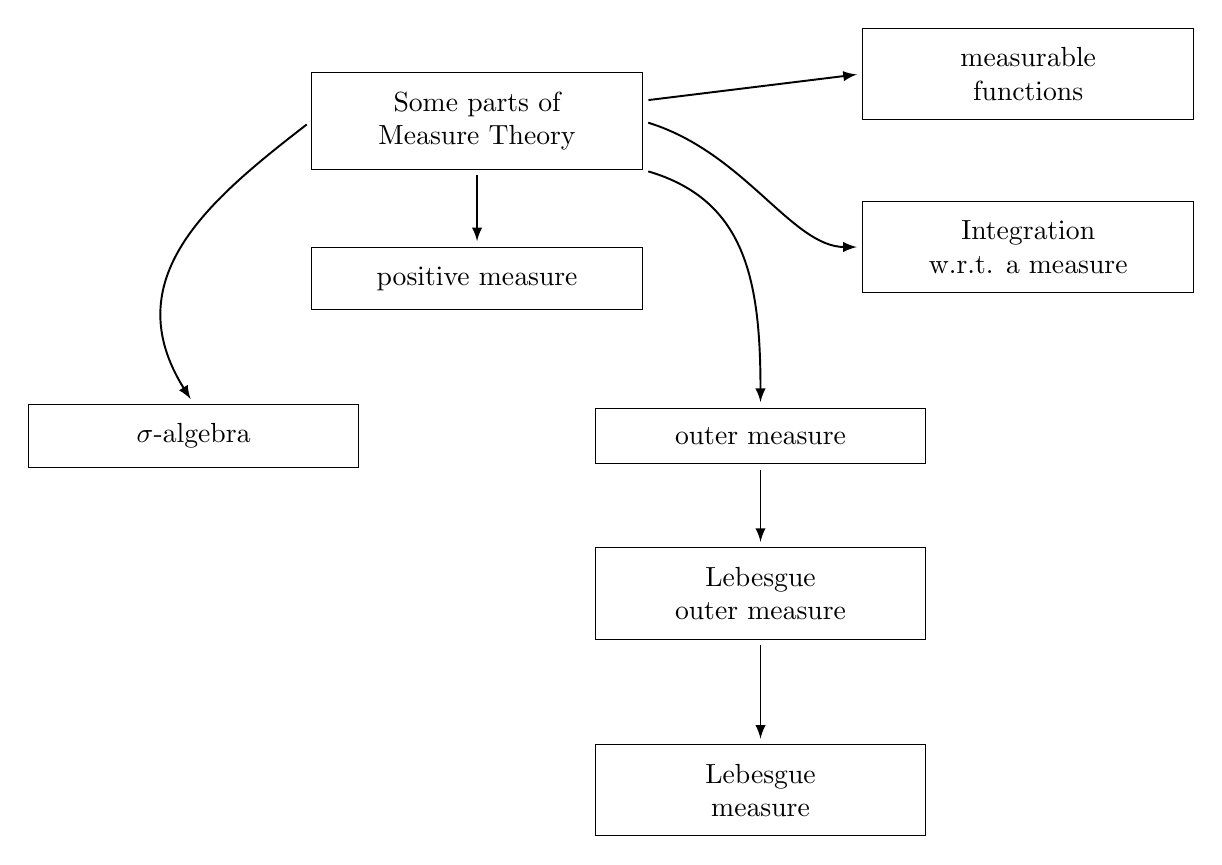
\begin{tikzpicture}[
    box/.style={
      rectangle, draw, align=center,
      inner sep=7pt, minimum width=4.2cm, font=\normalsize
    },
    >=latex, % arrowheads
    arrow/.style={->, shorten >=2pt, shorten <=2pt, line width=0.7pt},
  ]

  % Root (top)
  \node[box] (root) at (0,0) {Some parts of\\Measure Theory};

  % First row (closer to root; short connectors)
  \node[box] (sigma)   at (-3.6,-4) {$\sigma$-algebra};
  \node[box] (measure) at (0.0,-2)  {positive measure};
  \node[box] (outer)   at (3.6,-4)  {outer measure};

  % Right column (kept right and a bit higher/lower so it reads well)
  \node[box] (measurable) at (7.0,0.6)  {measurable\\functions};
  \node[box] (integration) at (7.0,-1.6) {Integration\\w.r.t. a measure};

  % Lower rows (longer vertical chain; avoids merging)
  \node[box] (lebesgueouter) at (3.6,-6) {Lebesgue\\outer measure};
  \node[box] (lebesgue)      at (3.6,-8.5) {Lebesgue\\measure};

  % Short, straight arrows for close children
  \draw[arrow] (root) -- (measure);
  \draw[arrow] (root) -- (measurable.west);

  % Long, routed arrow to the right column (clears the top and middle boxes)
  \draw[arrow] (root.east) .. controls (3.4,-0.4) and (4,-1.6) .. (integration.west);
  \draw[arrow] (root.west) .. controls (-3.4,-1) and (-4.6,-2) .. (sigma.north);
  \draw[arrow] (root) ..controls (3.4,-1) and (3.6,-2) .. (outer.north);

  % outer -> lebesgueouter -> lebesgue (longer downward chain so boxes are separate)
  \draw[arrow] (outer.south) -- ++(0,-0.45) -- (lebesgueouter.north);
  \draw[arrow] (lebesgueouter.south) -- ++(0,-0.45) -- (lebesgue.north);

\end{tikzpicture}
\end{center}


Let \( X \) be a set and \( \mathcal{P}(X) \) be its power set.

\begin{definition}[Algebra]
A collection \( \mathcal{A} \subseteq \mathcal{P}(X) \) is called an \textbf{algebra} (algebra of sets) if
\begin{itemize}
    \item \( \mathcal{A} \) is closed under finite union, i.e., \( E_{1},\ldots,E_{n} \in \mathcal{A} \implies \bigcup_{i=1}^{n} E_{i} \in \mathcal{A} \)
    \item \( E \in \mathcal{A} \implies E^{c} \in \mathcal{A} \)
\end{itemize}
\end{definition}

\begin{remark}
\begin{itemize}
    \item \( \emptyset, X \in \mathcal{A} \)
    \item \( \mathcal{A} \) is closed under finite intersection
\end{itemize}
\end{remark}

\begin{definition}[$\sigma$-algebra]
An algebra \( \mathcal{A} \subseteq \mathcal{P}(X) \) is called a \textbf{$\sigma$-algebra} if \( \mathcal{A} \) is closed under countable union, i.e.,
\[
E_{1},E_{2},\ldots \in \mathcal{A} \implies \bigcup_{n=1}^{\infty} E_{i} \in \mathcal{A}.
\]
\end{definition}

\begin{example}
Check that \( \mathcal{A} \) is a \(\sigma\)-algebra for the following:
\begin{enumerate}
    \item \( \mathcal{A} = \mathcal{P}(X) \)
    \item \( \mathcal{A} = \{E \in \mathcal{P}(X) : E \text{ is countable or } E^{c} \text{ is countable}\} \)
\end{enumerate}
Observe that intersection of any family of \(\sigma\)-algebras is also a \(\sigma\)-algebra.
\end{example}

\begin{definition}[$\sigma$-algebra generated by a set]
Let \( S \subseteq \mathcal{P}(X) \). Then the smallest \(\sigma\)-algebra containing \( S \) is called the \textbf{$\sigma$-algebra generated by $S$}, denoted by \( M(S) \).
\end{definition}

\begin{lemma}
Let \( S, F \subseteq \mathcal{P}(X) \) and \( S \subseteq M(S) \). Then \( M(S) \subseteq M(F) \).
\end{lemma}

\begin{proof}
Observe.
\end{proof}

\begin{definition}[Borel $\sigma$-algebra]
Let \( X \) be a topological space and \( S \) be the collection of all open sets in \( X \). The \(\sigma\)-algebra generated by \( S \) is the \textbf{Borel $\sigma$-algebra} on \( X \). We denote it by \( \mathcal{B}_{X} \). So \( \mathcal{B}_{X} \) induces at least the following sets:
\begin{enumerate}
    \item All open subsets of \( X \)
    \item All closed subsets of \( X \)
    \item Countable union of closed sets
    \item Countable intersection of open sets
\end{enumerate}
\end{definition}

\begin{proposition}
\( \mathcal{B}_{\mathbb{R}} \) is generated by any of the following:
\begin{enumerate}
    \item \( S_{1} = \{(a,b) : a < b\} \)
    \item \( S_{2} = \{[a,b] : a < b\} \)
    \item \( S_{3} = \{(a,b] : a < b\} \)
    \item \( S_{4} = \{[a,b) : a < b\} \)
    \item \( S_{5} = \{(-\infty,a) : a \in \mathbb{R}\} \)
    \item \( S_{6} = \{(a,\infty) : a \in \mathbb{R}\} \)
    \item \( S_{7} = \{(-\infty,a] : a \in \mathbb{R}\} \)
    \item \( S_{8} = \{[a,\infty) : a \in \mathbb{R}\} \)
\end{enumerate}
\end{proposition}

\begin{proof}
Let \( S \) be the collection of all open sets in \( \mathbb{R} \). Then
\[
S_{1} \subseteq S \implies M(S_{1}) \subseteq M(S).
\]
Also,
\[
S \subseteq M(S_{1}) \implies M(S) \subseteq M(S_{1}).
\]
Thus \( M(S_{1}) = M(S) = \mathcal{B}_{\mathbb{R}} \). Now notice that
\[
\bigcup_{n \geq 1} \left[a + \frac{1}{n}, b - \frac{1}{n}\right] = (a,b).
\]
Thus
\[
S_{2} \subseteq M(S_{1}) \implies M(S_{2}) \subseteq M(S_{1})
\]
and
\[
S_{1} \subseteq M(S_{2}) \implies M(S_{1}) \subseteq M(S_{2}).
\]
Thus \( M(S_{1}) = M(S_{2}) = \mathcal{B}_{\mathbb{R}} \). Do the rest similarly.
\end{proof}

\begin{definition}[Measure]
Let \( M \) be a \(\sigma\)-algebra on a set \( X \). A function \( \mu : M \mapsto [0,\infty) \) is said to be a \textbf{measure} if
\begin{enumerate}
    \item \( \mu(\emptyset) = 0 \)
    \item If \( \{E_{i}\}_{i \in \mathbb{N}} \) is a disjoint collection of sets in \( M \), then
    \[
    \mu\left( \bigcup_{i=1}^{\infty} E_{i} \right) = \sum_{i=1}^{\infty} \mu(E_{i})
    \]
\end{enumerate}
\( (X, M, \mu) \) is called a \textbf{measure space} and elements of \( M \) are called \textbf{measurable sets}.
\end{definition}

\begin{definition}[$\sigma$-Finite Measure Space]
A measure space \( (X, M, \mu) \) is said to be a \textbf{$\sigma$-finite measure space} if there exists a disjoint collection \( \{E_{i}\}_{i \in \mathbb{N}} \subseteq M \) such that \( X = \bigcup_{i=1}^{\infty} E_{i} \) and \( \mu(E_{i}) < \infty \).
\end{definition}

\begin{example}
\begin{enumerate}
    \item \textbf{Counting Measure:} \( (X, \mathcal{P}(X), \mu) \) such that \( \mu(E) = |E|  \forall  E \in \mathcal{P}(X) \). Check that \( \mu \) is a measure.
    \item \textbf{Dirac Measure:} Fix \( x_{0} \in X \). \( (X, \mathcal{P}(X), \mu) \) such that 
    \[
    \mu(E) = \begin{cases}
    0, & x_{0} \notin E \\
    1, & x_{0} \in E
    \end{cases}
    \]
    Check that \( \mu \) is a measure.
    \item Say \( x_{0}, y_{0} \in X \). Then 
    \[
    \mu(E) = \begin{cases}
    0, & x_{0}, y_{0} \notin E \\
    1, & x_{0} \text{ or } y_{0} \in E
    \end{cases}
    \]
    Check whether \( \mu \) is a measure.
\end{enumerate}
\end{example}

\endgroup


\newpage
\section{Lecture - 25/08/2025}

\textbf{Covered:} TBD

\begingroup
\setlength{\parskip}{6pt}
\setlength{\parindent}{0pt}

\begin{example}
For \( f: X \mapsto [0, \infty] \),
\[
\mu(E) = \sum_{x \in E} f(x)
\]
is a valid measure.
\end{example}

\begin{theorem}
Let \( \mu \) be a measure on \( \mathcal{M} \). Then

\begin{enumerate}[label=(\arabic*)]
    \item (Monotonicity) If \( E, F \in \mathcal{M} \) and \( E \subseteq F \),
    \[
    \mu(E) \leq \mu(F).
    \]
    
    \item (Countable sub-additivity) If \( \{E_i\}_{i \in \mathbb{N}} \subseteq \mathcal{M} \),
    \[
    \mu\left( \bigcup_{i=1}^{\infty} E_i \right) \leq \sum_{i=1}^{\infty} \mu(E_i).
    \]
    
    \item (Continuity from below) If \( E_1 \subseteq E_2 \subseteq \ldots \) and \( E_i \in \mathcal{M} \),
    \[
    \mu\left( \bigcup_{i=1}^{\infty} E_i \right) = \lim_{n \to \infty} \mu(E_n).
    \]
    
    \item (Continuity from above) If \( \{E_i\} \subseteq \mathcal{M} \) such that \( \mu(E_1) < \infty \) and \( E_1 \supseteq E_2 \supseteq \ldots \),
    \[
    \mu\left( \bigcap_{i=1}^{\infty} E_i \right) = \lim_{n \to \infty} \mu(E_n).
    \]
\end{enumerate}
\end{theorem}

\begin{proof}
\begin{enumerate}[label=(\arabic*)]
    \item \( F = E \cup (F \setminus E) \). Then \( \mu(F) = \mu(E) + \mu(F \setminus E) \geq \mu(E) \).
    
    \item Let
    \begin{align*}
    F_1 &= E_1, \\
    F_2 &= E_2 \setminus E_1, \\
    &\vdots \\
    F_k &= E_k \setminus \bigcup_{i=1}^{k-1} E_i.
    \end{align*}
    Then \( \bigcup_{k=1}^{\infty} F_k = \bigcup_{k=1}^{\infty} E_k \) and \( \{F_k\} \) is a disjoint family in \( \mathcal{M} \). So,
    \[
    \mu\left( \bigcup_{k=1}^{\infty} E_k \right) = \mu\left( \bigcup_{k=1}^{\infty} F_k \right) = \sum_{k=1}^{\infty} \mu(F_k) \leq \sum_{k=1}^{\infty} \mu(E_k),
    \]
    as \( F_k \subseteq E_k \) for all \( k \in \mathbb{N} \).
    
    \item Let \( E_0 = \emptyset \). Then
    \[
    \mu\left( \bigcup_{i=1}^{\infty} (E_i \setminus E_{i-1}) \right) = \sum_{i=1}^{\infty} \mu(E_i \setminus E_{i-1}) = \lim_{n \to \infty} \sum_{i=1}^{n} \mu(E_i \setminus E_{i-1}) 
    \]
    \[
    = \lim_{n \to \infty} \mu\left( \bigcup_{i=1}^{n} (E_i \setminus E_{i-1}) \right) = \lim_{n \to \infty} \mu(E_n).
    \]
    
    \item Define \( F_i = E_1 \setminus E_i \) for all \( i \). Then \( F_1 \subseteq F_2 \subseteq \ldots \). Also,
    \[
    \mu(F_i) = \mu(E_1) - \mu(E_i), \quad \text{i.e.,} \quad \mu(E_1) = \mu(F_i) + \mu(E_i).
    \]
    Then
    \[
    \mu\left( \bigcup_{i=1}^{\infty} F_i \right) = \lim_{n \to \infty} \mu(F_n) = \lim_{n \to \infty} [\mu(E_1) - \mu(E_n)]. \tag{16}
    \]
    Also,
    \[
    \bigcup_{i=1}^{\infty} F_i = E_1 \setminus \bigcap_{i=1}^{\infty} E_i \implies \mu\left( \bigcup_{i=1}^{\infty} F_i \right) + \mu\left( \bigcap_{i=1}^{\infty} E_i \right) = \mu(E_1).
    \]
    From (16),
    \[
    \mu(E_1) - \mu\left( \bigcap_{i=1}^{\infty} E_i \right) = \mu(E_1) - \lim_{n \to \infty} \mu(E_n) \implies \mu\left( \bigcap_{n=1}^{\infty} E_n \right) = \lim_{n \to \infty} \mu(E_n),
    \]
    as \( \mu(E_1) < \infty \). Instead of \( \mu(E_1) < \infty \), if we assume \( \mu(E_n) < \infty \) for some \( n \in \mathbb{N} \), then also (4) (\( \bigcap E_i = \bigcap_{i=n}^{\infty} E_i \)) is true.
    
    \[
    E_1 \supseteq E_2 \supseteq \ldots
    \]
    \( E_n = \{j \in \mathbb{N} : j \geq n\} \), \( \mu(E_n) = \infty \), \( \mu\left( \bigcap_{n \geq 1} E_n \right) = \mu(\emptyset) = 0 \). Let \( A_n = \mathbb{R}^+ \setminus [n, n+1] \), \( E_1 = A_1 \), \( E_2 = A_1 \cap A_2 \).
\end{enumerate}
\end{proof}

\begin{definition}[Null Set]
A set \( E \in \mathcal{M} \) is said to be a \textbf{null set} (measure zero set) if \( \mu(E) = 0 \). If a property holds on \( X \) except on a set of measure 0, we say that the property holds \textbf{almost everywhere} on \( X \). Say \( f = g \) on \( E^c \) where \( \mu \) is some Borel measure. Then we say \( f = g \) a.s.
\end{definition}

Say \( N \in \mathcal{M} \) and \( \mu(N) = 0 \) and \( F \subseteq N \).

\begin{definition}{Complete Measure}
Let \( (X, \mathcal{M}, \mu) \) be a measure space. \( \mu \) is said to be a \textbf{complete measure} if whenever \( F \subset N \) and \( \mu(N) = 0 \), \( F \in \mathcal{M} \).
\end{definition}

\begin{theorem}
Let \( (X, \mathcal{M}, \mu) \) be a measure space. Define
\[
\tilde{\mathcal{M}} = \{ E \cup F : E \in \mathcal{M} \text{ and } F \subset N \text{ where } N \text{ is a null set} \}.
\]
Then \( \tilde{\mathcal{M}} \) is a \( \sigma \)-algebra and there is an extension of \( \mu \) to \( \tilde{\mathcal{M}} \) such that \( \tilde{\mu} \) is a complete measure.
\end{theorem}

\begin{proof}
\[
\bigcup_{i \geq 1} (E_i \cup F_i) = \left( \bigcup_{i \geq 1} E_i \right) \cup \left( \bigcup_{i \geq 1} F_i \right) \in \tilde{\mathcal{M}}.
\]
We have to check if
\[
E \cup F \in \tilde{\mathcal{M}} \implies (E \cup F)^c \in \tilde{\mathcal{M}}.
\]
We can always assume \( E \cap N = \emptyset \). Then
\[
E \cup F = E \cup (F \setminus E).
\]
Now, \( E \cap (N \setminus E) = \phi \). Then
\[
E \cup F = (E \cup N) \setminus (N \setminus F) = (E \cup N) \cap [(N \cap F^c)^c] = (E \cup N) \cap (F \cup N^c).
\]
Thus
\[
(E \cup F)^c = (E \cup N)^c \cup (N \setminus F^c).
\]
So \( \tilde{\mathcal{M}} \) is a \( \sigma \)-algebra. Define
\[
\tilde{\mu}(E \cup F) = \mu(E) \quad \forall E \cup F \in \tilde{\mathcal{M}}.
\]

\textbf{Well-definedness of \( \tilde{\mu} \):} Let \( E_1 \cup F_1 = E_2 \cup F_2 \) for \( E_1, E_2 \in \mathcal{M} \), \( F_1 \subset N_1 \), \( F_2 \subset N_2 \). Then
\[
E_1 \subseteq E_2 \cup F_2 \subseteq E_2 \cup N_2 \implies \mu(E_1) \leq \mu(E_2) + \mu(N_2) = \mu(E_2).
\]
Similarly, \( \mu(E_2) \leq \mu(E_1) \implies \mu(E_1) = \mu(E_2) \). Check that \( \tilde{\mu} \) is a measure. Also, it is complete.
\end{proof}

\textbf{Outer Measure:} Let \( X \) be a set. A function
\[
\mu^* : \mathcal{P}(X) \mapsto [0, \infty]
\]
is called an \textbf{outer measure} if

\begin{enumerate}[label=(\arabic*)]
    \item \( \mu^*(\emptyset) = 0 \)
    \item \( A \subseteq B \implies \mu^*(A) \leq \mu^*(B) \)
    \item \( \mu^* \) is countably sub-additive, i.e., \( \mu^*\left( \bigcup_{i=1}^{\infty} E_i \right) \leq \sum_{i=1}^{\infty} \mu^*(E_i) \).
\end{enumerate}

\begin{theorem}
Let \( \Sigma \subseteq \mathcal{P}(X) \) and \( \rho : \Sigma \mapsto [0, \infty] \) such that \( \emptyset, X \in \Sigma \) and \( \rho(\emptyset) = 0 \). We define for all \( E \subseteq X \),
\[
\mu^*(E) = \inf \left\{ \sum_{i=1}^{\infty} \rho(E_i) \mid E \subset \bigcup_{i=1}^{\infty} E_i, E_i \in \Sigma \right\}.
\]
Then \( \mu^* \) is an outer measure on \( X \).
\end{theorem}

\begin{proof}
The definition of \( \mu^* \) makes sense as \( \mu^*(\emptyset) = 0 \), \( \mu^*(A) \leq \mu^*(B) \) for \( A \subseteq B \). Let \( \{A_i\}_{i \in \mathbb{N}} \subseteq \mathcal{P}(X) \). We need to show that
\[
\mu^*\left( \bigcup_{i=1}^{\infty} A_i \right) \leq \sum_{i=1}^{\infty} \mu^*(A_i).
\]
Let \( \epsilon > 0 \). For each \( i \in \mathbb{N} \), there exists \( \{E_{ik}\}_{k \in \mathbb{N}} \) such that
\[
\sum_{k=1}^{\infty} \rho(E_{ik}) \leq \mu^*(A_i) + \frac{\epsilon}{2^i} 
\]
\[
\implies \sum_{i=1}^{\infty} \sum_{k=1}^{\infty} \rho(E_{ik}) \leq \sum_{i=1}^{\infty} \mu^*(A_i) + \epsilon \left( \frac{1}{2} + \frac{1}{2^2} + \ldots \right) 
\]
\[
\implies \mu^*\left( \bigcup_{i \geq 1} A_i \right) \leq \sum_{i} \sum_{k} \rho(E_{ik}) \leq \sum_{i} \mu^*(A_i) + \epsilon 
\]
\[
\implies \mu^*\left( \bigcup_{i \geq 1} A_i \right) \leq \sum_{i \geq 1} \mu^*(A_i).
\]
\end{proof}

\begin{theorem}[Carathéodory's Theorem]
Let \( \mu^* \) be an outer measure on \( X \) and \( \mathcal{M} \) be the collection of all \( \mu^* \)-measurable sets. Then \( \mathcal{M} \) is a \( \sigma \)-algebra and \( \mu^* \) is a measure on \( \mathcal{M} \).
\end{theorem}

\endgroup


\newpage
\section{Lecture - 01/09/2025}

\textbf{Covered:} TBD

\begingroup
\setlength{\parskip}{6pt}
\setlength{\parindent}{0pt}

\begin{theorem}[Caratheodory's Theorem]
Let $X$ be a set and $\mu^{*}$ be an outer measure on $X$ and $\mathcal{M}$ be the collection of all $\mu^{*}$-measurable sets. Then $\mathcal{M}$ is a $\sigma$-algebra and $\mu^{*}$ is a measure on $\mathcal{M}$.

$A \subseteq \mathcal{P}(X)$ is said to be $\mu^{*}$-measurable if

\[
\mu^{*}(E) = \mu^{*}(E \cap A) + \mu^{*}(E \cap A^{c}) \ \forall\ E \subseteq X.
\]
\end{theorem}

\begin{proof}
It is clear that if $A$ is $\mu^{*}$-measurable then so is $A^{c}$. Let $A,B \in \mathcal{M}\ \forall\ E \subseteq X$. Then

\[
\mu^{*}(E) = \mu^{*}(E \cap A) + \mu^{*}(E \cap A^{c}) \ (\because\ A \in \mathcal{M})
\]

\[
= \mu^{*}(E \cap A \cap B) + \mu^{*}(E \cap A \cap B^{c}) + \mu^{*}(E \cap A^{c} \cap B) + \mu^{*}(E \cap A^{c} \cap B^{c})
\]

\[
\geq \mu^{*}(E \cap (A \cup B)) + \mu^{*}(E \cap (A \cup B)^{c})\ [\text{ctbl. subadd.}]
\]

Also we clearly have

\[
\mu^{*}(E) \leq \mu^{*}(E \cap (A \cup B)) + \mu^{*}(E \cap (A \cup B)^{c}) \implies A \cup B \in \mathcal{M}.
\]

If $A,B \in \mathcal{M}\ \&\ A \cap B = \emptyset$, then

\[
\mu^{*}(A \cup B) = \mu^{*}(A \cup B \cap A) + \mu^{*}(A \cup B \cap A^{c}) = \mu^{*}(A) + \mu^{*}(B).
\]

Fact: Any $\sigma$-algebra $\mathcal{M}$ is closed under countable disjoint union. Countable union $\implies$ Countable disjoint union is obvious as it includes all kinds of countable. For converse, take $\{E_{i}\}$ collection in $\mathcal{M}$. We define $F_{1} = E_{1}\ \&\ F_{n} = E_{n} \setminus \bigcup_{i=1}^{n-1} E_{i}$ which is a disjoint family such that $\bigcup_{i=1}^{n} F_{i} = \bigcup_{i=1}^{n} E_{i}$. So $\bigcup_{i=1}^{\infty} E_{i} \in \mathcal{M}$ is closed under countable disjoint union. Now we will see $\mathcal{M}$ is closed under disjoint union. Let $\{E_{i}\}$ be a countable disjoint collection set,

\[
B_{n} = \bigcup_{i=1}^{n} E_{i},\ B = \bigcup_{i=1}^{\infty} E_{i}.
\]

By the first part, $B_{n}$ is $\mu^{*}$-measurable, i.e., $\forall\ E \subseteq X$,

\[
\mu^{*}(E) = \mu^{*}(E \cap B_{n}) + \mu^{*}(E \cap B_{n}^{c})
\]

\[
= \mu^{*}(E \cap B_{n} \cap E_{n}) + \mu^{*}(E \cap B_{n} \cap E_{n}^{c}) + \mu^{*}(E \cap B_{n}^{c})
\]

\[
= \mu^{*}(E \cap E_{n}) + \mu^{*}(E \cap E_{n-1}) + \mu^{*}(E \cap B_{n-2}) + \mu^{*}(E \cap B_{n}^{c})
\]

\[
= \sum_{i=1}^{n} \mu^{*}(E \cap E_{n}^{c}) + \mu^{*}(E \cap B_{n}^{c}) \geq \sum_{i=1}^{n} \mu^{*}(E \cap E_{n}^{c}) + \mu^{*}(E \cap B^{c})\ (\because\ B_{n}^{c} \supseteq B^{c}).
\]

Taking $n \to \infty$, we get

\[
\mu^{*}(E) \geq \sum_{i=1}^{\infty} \mu^{*}(E \cap E_{i}) + \mu^{*}(E \cap B^{c}) \geq \mu^{*}(E \cap B) + \mu^{*}(E \cap B^{c}) \geq \mu^{*}(E). \tag{17}
\]

$\therefore B$ is $\mu^{*}$-measurable, i.e., $B \in \mathcal{M}$. From (17),

\[
\mu^{*}(E \cap B) = \sum_{i=1}^{\infty} \mu^{*}(E \cap E_{i}).
\]

In particular, take $E = B$,

\[
\mu^{*}(B) = \sum_{i=1}^{\infty} \mu^{*}(E_{i})\ \text{ctbl. additive}.
\]

$\therefore \mu^{*}$ is a measure on $\mathcal{M}$. It remains to show that $\mu^{*}$ is a complete measure. Take $A \subseteq X$ s.t. $\mu^{*}(A) = 0$. Then

\[
\mu^{*}(E) \leq \mu^{*}(E \cap A) + \mu^{*}(E \cap A^{c}) = \mu^{*}(E \cap A^{c}) \leq \mu^{*}(E).
\]

Therefore

\[
\mu^{*}(E) = \mu^{*}(E \cap A) + \mu^{*}(E \cap A^{c})\ \forall\ E \subseteq X
\]

$\implies\ A \in \mathcal{M}.$ By the above, all the subsets $B \subseteq A$ also belong to $\mathcal{M}.$ Therefore $\mu^{*}$ is a complete measure on $\mathcal{M}$.
\end{proof}

\begin{definition}[Premeasure]
Let $\mathcal{A} \subseteq \mathcal{P}(X)$ be an algebra. A \textbf{premeasure} $\mu_{0}$ is a function $\mu_{0} : \mathcal{A} \mapsto [0,1]$ s.t.

\begin{itemize}
    \item $\mu_{0}(\emptyset) = 0$
    \item $(E_{i})$ countable disjoint collection s.t. $\bigcup_{i=1}^{\infty} E_{i} \in \mathcal{A}.$ Then
    \[
    \mu_{0}\left(\bigcup_{i=1}^{\infty} E_{i}\right) = \sum_{i=1}^{\infty} \mu_{0}(E_{i}).
    \]
\end{itemize}

We can define an outer measure by following:

\[
\mu^{*}(E) = \inf\left\{\sum_{i=1}^{\infty} \mu_{0}(A_{i}) \mid E \subseteq \bigcup_{i=1}^{\infty} A_{i},\ A_{i} \in \mathcal{A}\right\}.
\]
\end{definition}

\begin{proposition}
Let $\mu_{0}$ be a premeasure on an algebra $\mathcal{A} \subseteq \mathcal{P}(X).$ Then there is an outer measure $\mu^{*}$ s.t.

\begin{enumerate}
    \item $\mu^{*} \mid_{\mathcal{A}} = \mu_{0}$
    \item Every set in $\mathcal{A}$ is $\mu^{*}$-measurable
\end{enumerate}
\end{proposition}

\begin{proof}
\begin{enumerate}
    \item Suppose $E \in \mathcal{A}.$ Then $E \subseteq \bigcup_{i=1}^{\infty} A_{i},\ A_{i} \in \mathcal{A}.$ Then $B_{n} := E \cap \left(A_{n} \setminus \bigcup_{i=1}^{n-1} A_{i}\right)$ is a disjoint collection and $E = \bigcup_{i=1}^{\infty} B_{n}.$ So
    \[
    \mu_{0}(E) = \sum_{i=1}^{\infty} \mu_{0}(B_{n}) \leq \sum_{n=1}^{\infty} \mu_{0}(A_{n}).
    \]
    $\therefore\ \mu_{0}(E) \leq \mu^{*}(E).$ Taking $A_{1} = E$ and $A_{i} = \emptyset\ \forall\ i \neq 1$,
    \[
    \mu^{*}(E) = \mu_{0}(E).
    \]
    Thus $\mu^{*}(E) = \mu_{0}(E)\ \forall\ E \in \mathcal{A}$.
    
    \item Let $A \in \mathcal{A},\ E \subseteq X,\ \epsilon > 0.$ Then $\exists$ a sequence $\{B_{i}\}$ s.t. $E \subseteq \bigcup_{i=1}^{\infty} B_{i}$.
    \[
    \sum_{i=1}^{\infty} \mu_{0}(B_{i}) \leq \mu^{*}(E) + \epsilon \implies \sum_{i=1}^{\infty} \mu_{0}(B_{i} \cap A) + \sum_{i=1}^{\infty} \mu_{0}(B_{i} \cap A^{c}) \leq \mu^{*}(E) + \epsilon
    \]
    \[
    \implies \mu^{*}(E \cap A) + \mu^{*}(E \cap A^{c}) \leq \sum_{i=1}^{\infty} \mu_{0}(B_{i} \cap A) + \sum_{i=1}^{\infty} \mu_{0}(B_{i} \cap A^{c}) \leq \mu_{0}^{*}(E) + \epsilon
    \]
    \[
    \implies \mu^{*}(E \cap A) + \mu^{*}(E \cap A^{c}) \leq \mu^{*}(E)\ \text{(for some arbitrary $\epsilon$)}.
    \]
    So
    \[
    \mu^{*}(E) = \mu^{*}(E \cap A) + \mu^{*}(E \cap A^{c})
    \]
    or $A$ is $\mu^{*}$-measurable.
\end{enumerate}
\end{proof}

\begin{theorem}
Let $\mathcal{A} \in \mathcal{P}(X)$ be an algebra, $\mu_{0}$ be a premeasure on $\mathcal{A}$ and $\mathcal{M}$ be the $\sigma-$algebra generated by $\mathcal{A}$. Then

\begin{enumerate}
    \item There exists a measure $\mu$ on $\mathcal{M}$ whose restriction to $\mathcal{A}$ in $\mu_{0}$ (basically $\mu = \mu^{*} \mid_{\mathcal{M}}$, $\mu^{*}$ is the $\inf$ formula)
    \item If $v$ is another measure on $\mathcal{M}$ that extends $\mu_{0}$ then $v(E) \leq \mu(E)\ \forall\ E \in \mathcal{M}$.
    \item The equality above holds if $\mu(E) < \infty$.
    \item If $\mu_{0}$ is $\sigma-$finite then $\mu$ is the unique extension of $\mu_{0}$ to a measure on $\mathcal{M}$.
\end{enumerate}
\end{theorem}

\begin{proof}
\begin{enumerate}
    \item Uses Caratheodory's theorem and the previous proposition. Let $\mathcal{M}^{\prime}$ be the set of all $\mu^{*}-$measurable sets where $\mu^{*}$ comes from $\mu_{0}$. Then by Caratheodory's theorem, $\mu^{*} \mid_{\mathcal{M}} = \mu_{0}$. By previous proposition,
    \[
    \mu^{*} \mid \mathcal{A} = \mu_{0} \implies \mu^{*} \mid_{\mathcal{M}} = \mu_{0}
    \]
    as $\mathcal{M}(A) = \mathcal{M} \subseteq \mathcal{M}^{\prime}$
    
    \item Let $E \in \mathcal{M}$ and $E = \bigcup_{i=1}^{\infty} A_{i},\ A_{i} \in \mathcal{A}$. Then
    \[
    v(E) \leq \sum_{i=1}^{\infty} \mu(A_{i}) = \sum_{i=1}^{\infty} \mu_{0}(A_{i})
    \]
    \[
    \implies v(E) = \mu^{*}(E) = \mu(E).
    \]
    
    \item If $A = \bigcup_{i=1}^{\infty} A_{i}$,
    \[
    v(A) = \lim_{n \to \infty} v\left(\bigcup_{i=1}^{n} A_{i}\right) = \lim_{n \to \infty} \mu\left(\bigcup_{i=1}^{n} A_{i}\right) = \mu(A).
    \]
    
    \item $X = \bigcup_{i=1}^{m} A_{i}$ s.t. $\{A_{i}\}_{i \in \mathbb{N}}$ is a disjoint collection and $v_{0}(A_{i}) < \infty.$ Then for $E \in \mathcal{M}$,
    \[
    \mu(E) = \sum_{i=1}^{\infty} \mu(E \cap A_{i}) = \sum_{i=1}^{\infty} v(E \cap A_{i}) = v(E).
    \]
\end{enumerate}
\end{proof}

\begin{remark}
Basically, through the same procedure we get a measure on the $\sigma-$algebra of $\mu^{*}$ measurable sets that extends $\mu_{0}$.
\end{remark}

\subsection{Construction of Lebesgue Measure} Let

\[
\mathcal{A} = (\text{finite disjoint union of } \{\text{intervals in } \mathbb{R}\}_{\subseteq} \mathcal{B}_{\mathbb{R}}.
\]

\noindent\textbf{Exercise:} $\mathcal{A}$ is an algebra.

\begin{proposition}
Let $\{(a_{i},b_{i})\}_{i=1}^{n}$ be any disjoint collection in $\mathcal{A}.$ Define

\[
\mu_{0}\left(\bigcup_{i=1}^{n} (a_{i},b_{i})\right) = \sum_{i=1}^{n} (b_{i} - a_{i}),\ \mu_{0}(\emptyset) = 0 \implies
\]

$\mu_{0}$ is a premeasure on $\mathcal{A}.$
\end{proposition}

\begin{proof}
Let $\{I_{i}\}_{i=1}^{n}$ and $\{J_{j}\}_{j=1}^{m}$ be two disjoint collections of h-proper intervals. Then

\[
\sum_{i=1}^{n} I_{i} = \sum_{j=1}^{m} J_{j} \implies \mu_{0}\left(\bigcup_{i=1}^{n} I_{i}\right) = \sum_{i=1}^{n} \mu_{0}(I_{i}) = \sum_{j=1}^{m} \sum_{i=1}^{n} \mu_{0}(I_{i} \cap J_{i})
\]

\[
= \sum_{j=1}^{m} \mu_{0}(J_{j}) = \mu_{0}\left(\bigcup_{j=1}^{m} J_{j}\right).
\]

So $\mu_{0}$ is well-defined. From the definition of $\mu_{0}$, it is clear that $\mu_{0}$ is finitely additive. Remains to prove, if $\bigsqcup_{i=1}^{\infty} I_{i} \in \mathcal{A}$ then $\mu_{0}(\bigcup_{i=1}^{\infty}) = \sum_{i=1}^{\infty} \mu_{0}(I_{i}).$ Since $\bigcup_{i=1}^{\infty} I_{i} \in A,\ \bigcup_{i=1}^{\infty} I_{i}$ is the finite disjoint union of h-intervals $\{J_{j}\}_{j=1}^{m}$, \textit{i.e.},

\[
J_{j} = \sum_{i=1}^{\infty} I_{j_{i}}\ \forall\ j \leq m
\]

where $\{J_{j_{i}}\}_{i=1}^{\infty}$ is some subsequence of $\{J_{i}\}_{i=1}^{\infty}$. Then

\[
\mu_{0}\left(\bigcup_{i=1}^{\infty} I_{i}\right) = \mu_{0}\left(\underbrace{\bigcup_{j=1}^{m} I_{j}}_{\in \mathcal{A}}\right) = \sum_{j=1}^{m} \mu_{0}(J_{j}) \left(\mu_{0}(J_{j}) = \sum_{i=1}^{\infty} \mu_{0}(I_{j_{i}})\right)
\]

\[
\geq \mu_{0}\left(\bigcup_{i=1}^{\infty} I_{j_{i}}\right) = \mu\left(J_{j} \setminus \sum_{i=1}^{n} I_{j_{i}}\right) \geq \sum_{i=1}^{n} \mu_{0}(I_{j_{i}})\ \forall\ n
\]

\[
\implies \mu_{0}(J_{j}) \geq \sum_{i=1}^{\infty} \mu_{0}(I_{j_{i}})\ \text{as}\ n \to \infty.
\]
\end{proof}

\endgroup

\newpage
\section{Lecture - 05/09/2025}

\textbf{Covered:} Joint Distributions contd., Independence

\begingroup
\setlength{\parskip}{6pt}
\setlength{\parindent}{0pt}

\textbf{Alternative Proof:}

\begin{enumerate}
    \item Let $\mu^{*}$ be the outer measure corresponding to $\mathcal{M}$ . Then take $\mu = \mu^{*} \mid_{\mathcal{M}}$ . Let $\mathcal{M}^{\prime}$ be the $\sigma-$algebra of $\mu^{*}$ measurable sets. Then obviously, $\mathcal{M} \subseteq \mathcal{M}^{\prime}$. Also, $\mu^{*} \mid_{\mathcal{M}^{\prime}}$ is a measure. So $\mu$ is a measure. Also, $\mu^{*} \mid_{\mathcal{A}} = \mu_{0} \implies \mu \mid_{\mathcal{A}} = \mu_{0}$.
    
    \item Let $E \in \mathcal{M}$. Then $E \subseteq \bigcup_{i=1}^{\infty} A_{i}$ where $A_{i} \in \mathcal{A}$. So
    \[
    v(E) \leq v\left(\bigcup_{i=1}^{\infty} A_{i}\right) \leq \sum_{i=1}^{\infty} v(A_{i}) = \sum_{i=1}^{\infty} \mu_{0}(A_{i})
    \]
    \[
    \implies v(E) \leq \mu^{*}(E) = \mu(E)\ (\text{taking inf on right side over all covers of } E).
    \]
    
    \item Let $A = \bigcup_{i=1}^{n} A_{i},\ A \in \mathcal{A}.$ Then
    \[
    v(A) = \lim_{n \to \infty} v\left(\bigcup_{i=1}^{n} A_{i}\right) = \lim_{n \to \infty} \mu\left(\bigcup_{i=1}^{n} A_{i}\right) = \mu(A).
    \]
    If $\mu(E) < \infty,$ then we can choose $A^{\prime}_{i}$s s.t.
    \[
    A = \bigcup_{i=1}^{\infty} A_{i},\ \mu(A) < \mu(E) + \epsilon
    \]
    and thus $\mu(A \setminus E) < \epsilon.$ Then
    \[
    \mu(E) \leq \mu(A) = v(A) = v(E) + v(A \setminus E) < v(E) + \mu(A \setminus E) < v(E) + \epsilon.
    \]
    Since $E$ arbitrary and $\mu(E) \leq v(E),\ \mu(E) = v(E).$
    
    \item $X = \bigcup_{i=1}^{m} A_{i}$ s.t. $\{A_{i}\}_{i \in \mathbb{N}}$ is a disjoint collection and $v_{0}(A_{i}) < \infty.$ Then for $E \in \mathcal{M}$,
    \[
    \mu(E) = \sum_{i=1}^{\infty} \mu(E \cap A_{i}) = \sum_{i=1}^{\infty} v(E \cap A_{i}) = v(E).
    \]
\end{enumerate}

\begin{remark}
Basically, through the same procedure we get a measure on the $\sigma-$algebra of $\mu^{*}$ measurable sets that extends $\mu_{0}$.
\end{remark}

\textbf{Construction of Lebesgue Measure:} Let

\[
\mathcal{A} = (\text{finite disjoint union of } \{\text{intervals in } \mathbb{R}\}_{\subseteq} \mathcal{B}_{\mathbb{R}}.
\]

\noindent\textbf{Exercise:}$\mathcal{A}$ is an algebra.

\begin{proposition}
Let $\{(a_{i},b_{i})\}_{i=1}^{n}$ be any disjoint collection in $\mathcal{A}.$ Define

\[
\mu_{0}\left(\bigcup_{i=1}^{n} (a_{i},b_{i})\right) = \sum_{i=1}^{n} (b_{i} - a_{i}),\ \mu_{0}(\emptyset) = 0 \implies
\]

$\mu_{0}$ is a premeasure on $\mathcal{A}.$
\end{proposition}

\begin{proof}
Let $\{I_{i}\}_{i=1}^{n}$ and $\{J_{j}\}_{j=1}^{m}$ be two disjoint collections of h-proper intervals. Then

\[
\sum_{i=1}^{n} I_{i} = \sum_{j=1}^{m} J_{j} \implies \mu_{0}\left(\bigcup_{i=1}^{n} I_{i}\right) = \sum_{i=1}^{n} \mu_{0}(I_{i}) = \sum_{j=1}^{m} \sum_{i=1}^{n} \mu_{0}(I_{i} \cap J_{i})
\]

\[
= \sum_{j=1}^{m} \mu_{0}(J_{j}) = \mu_{0}\left(\bigcup_{j=1}^{m} J_{j}\right).
\]

So $\mu_{0}$ is well-defined. From the definition of $\mu_{0}$, it is clear that $\mu_{0}$ is finitely additive. Remains to prove, if $\bigsqcup_{i=1}^{\infty} I_{i} \in \mathcal{A}$ then $\mu_{0}(\bigcup_{i=1}^{\infty}) = \sum_{i=1}^{\infty} \mu_{0}(I_{i}).$ Since $\bigcup_{i=1}^{\infty} I_{i} \in A,\ \bigcup_{i=1}^{\infty} I_{i}$ is the finite disjoint union of h-intervals $\{J_{j}\}_{j=1}^{m}$, \textit{i.e.},

\[
J_{j} = \sum_{i=1}^{\infty} I_{j_{i}}\ \forall\ j \leq m
\]

where $\{J_{j_{i}}\}_{i=1}^{\infty}$ is some subsequence of $\{J_{i}\}_{i=1}^{\infty}$. Then

\[
\mu_{0}\left(\bigcup_{i=1}^{\infty} I_{i}\right) = \mu_{0}\left(\underbrace{\bigcup_{j=1}^{m} I_{j}}_{\in \mathcal{A}}\right) = \sum_{j=1}^{m} \mu_{0}(J_{j}) \left(\mu_{0}(J_{j}) = \sum_{i=1}^{\infty} \mu_{0}(I_{j_{i}})\right)
\]

\[
\geq \mu_{0}\left(\bigcup_{i=1}^{\infty} I_{j_{i}}\right) = \mu\left(J_{j} \setminus \sum_{i=1}^{n} I_{j_{i}}\right) \geq \sum_{i=1}^{n} \mu_{0}(I_{j_{i}})\ \forall\ n
\]

\[
\implies \mu_{0}(J_{j}) \geq \sum_{i=1}^{\infty} \mu_{0}(I_{j_{i}})\ \text{as}\ n \to \infty.
\]
\end{proof}

\endgroup


\newpage
\section{Lecture - 15/09/2025}

\textbf{Covered:} TBD

\begingroup
\setlength{\parskip}{6pt}
\setlength{\parindent}{0pt}

We extend $\mu_{0}$ on $\mathcal{A}$ to $\mu$ on $\mathcal{M}$ to $\mu^{*}$ on $\mu^{\prime}$ where

\[
\mu^{*}(A) = \inf\left\{\sum_{A \in \mathcal{A}} \mu_{0}(A_{i}) \middle| A \subseteq \bigcup_{A_{i} \in \mathcal{A}} A_{i}\right\}.
\]

Then $\mathcal{M}^{\prime} = (\text{collection of } \mu^{*}-\text{measure sets}).$ We have that $\mu^{*}|_{\mathcal{M}^{\prime}}$ is a measure, $\mathcal{A} \subseteq \mathcal{M}^{\prime}.$ Let $\mathcal{M} = \mathcal{M}(\mathcal{A}) \implies \mathcal{M} \subseteq \mathcal{M}^{\prime}.$ Then $\mu^{*}$ is a measure on $\mathcal{M}$ which returns $\mu_{0}$ if $\mu_{0}$ is cofinite on $X.$ Then $\mu^{*}|_{\mathcal{M}}$ is a unique measure which extends $\mu_{0}.$ An h-interval is of the form $\{(-\infty,b],(a,b),(a,\infty)|a,b \in \mathbb{R}\}$ and $\mathcal{A} = (\text{finite disjoint unions of h-intervals})$ is an algebra.

\begin{proposition}
On $\mathcal{A}$ define $\mu_{0}$ by

\[
\mu_{0}\left(\bigsqcup_{i=1}^{n} (a_{i},b_{i})\right) = \sum_{i=1}^{n} (b_{i} - a_{i}).
\]

Then $\mu_{0}$ is a premeasure on $\mathcal{A}.$
\end{proposition}

\begin{proof}
Let $\{A_{i}\}_{i=1}^{\infty}$ is a countable disjoint collection of sets in $\mathcal{A}$ if $\bigsqcup_{i=1}^{\infty} A_{i} \in \mathcal{A}.$ We need to prove that $\mu_{0}(\bigsqcup_{j=1}^{\infty} A_{i}) = \sum_{i=1}^{\infty} \mu_{0}(A_{i}).$ Let $\bigsqcup_{i=1}^{\infty} A_{i} = \bigsqcup_{j=1}^{k} (a_{i},b_{j}]$ where $(a_{i},b_{j}] = \bigsqcup_{i,j}^{\infty} C_{ij}$ where $A_{i} = \bigsqcup_{j=1}^{\infty} C_{ij}.$ It is enough to show that

\[
\mu_{0}(a_{i},b_{j}] = \sum_{i=1}^{\infty} \mu_{0}(a_{j_{i}},b_{j_{i}}).
\]

Basically if $[a,b] = \bigsqcup_{i=1}^{\infty} (a_{i},b_{i}]$ then $\mu_{0}(a,b] = \sum_{j=1}^{\infty} \mu_{0}(a_{i},b_{i}]$. Then

\[
\bigsqcup_{i=1}^{\infty} [a_{i},b_{i}] = \bigsqcup_{i=1}^{N} [a_{i},b_{i}] + \bigsqcup_{i=N+1}^{\infty} (a_{i},b_{i}] \implies \mu_{0}\left(\bigsqcup_{i=1}^{\infty} [a_{i},b_{i}]\right) \geq \mu_{0}\left(\bigsqcup_{i=1}^{N} [a_{i},b_{i}]\right) = \sum_{i=1}^{N} \mu_{0}(a_{i},b_{i}].
\]

Taking $N \to \infty$,

\[
\mu_{0}(a,b] = \mu_{0}\left(\bigsqcup_{i=1}^{\infty} [a_{i},b_{i}]\right) \geq \sum_{i=1}^{\infty} \mu_{0}(a_{i},b_{i}].
\]

Choose $\epsilon > 0$ and take $\delta,\delta_{i}$ s.t. $\delta < \epsilon$, $\delta_{i} < \frac{\epsilon}{2^{i}}$. Then $[a+\delta,b] \subseteq \bigcup_{i=1}^{\infty} (a_{i},b_{i} + \delta_{i})$. Since $[a+\delta,b]$ is compact, $[a+\delta,b] = \bigcup_{i=1}^{N} (a_{i},b_{i} + \delta_{i})$. Now,

\[
\mu_{0}(a,b] = (b-a) \leq b-(a+\delta) + \epsilon \leq b_{N} + \delta_{N} - a_{1} + \epsilon
\]

\[
= b_{N} + \delta_{N} - a_{N} + \sum_{i=1}^{N-1} [a_{i+1} - a_{i}] + \epsilon \leq b_{N} + \delta_{N} - a_{N} + \sum_{i=1}^{N-1} [b_{i} + \delta_{i} - a_{i}]
\]

\[
< \sum_{i=1}^{N} (b_{i} - a_{i}) + \sum_{i=1}^{\infty} \delta_{N} + \epsilon < \sum_{i=1}^{\infty} (b_{i} - a_{i}) + \underbrace{\sum_{i=1}^{\infty} \frac{\epsilon}{2^{i}}}_{=2\epsilon} + \epsilon.
\]

As $\epsilon$ was arbitrary, $(b-a) \leq \sum_{i=1}^{\infty} (b-i - a_{i})$. Therefore, $\mu_{0}(a,b] = \sum_{i=1}^{\infty} \mu_{0}(a_{i},b_{i}]$. For intervals of type $(-\infty,b]$, $\forall\ M < \infty$ we look at $(-M,b)$ intervals. Let $(-\infty,b] = \sum_{i=1}^{N} (a_{i},b_{i}] \implies (-M,b) \subseteq \bigsqcup_{i=1}^{\infty} a_{i},b_{i}]$. Taking $M \to \infty$,

\[
\mu_{0}(-\infty,b] \leq \sum_{i=1}^{\infty} \mu_{0}(a_{i},b_{i}).
\]

Let $\mathcal{L} := [\mu^{*}-\text{measurable sets}]$, a Lebesgue $\sigma-$algebra. Lebesgue measure: Complete measure $m = \mu^{*}|_{\mathcal{L}}$ and $\mu = m|_{\mathcal{B}_{\mathbb{R}}}$ Then $\mathcal{B}_{\mathbb{R}} \subseteq \mathcal{L} \implies \bar{\mathcal{B}}_{\mathbb{R}} \subseteq \mathcal{L}$ as $\mathcal{A} \subseteq \mathcal{L} \implies \mathcal{B}_{\mathbb{R}} = \mathcal{M}(\mathcal{A}) \subseteq \mathcal{L}$. \textbf{Question:} Is $\bar{\mathcal{B}}_{\mathbb{R}} = \mathcal{L}$?
\end{proof}

\begin{proposition}
Let $E \in \mathcal{L}$. Then

\[
m(E) = \inf\left\{\sum_{i=1}^{\infty} m(a_{i},b_{i}) \middle| E \subseteq \bigcup_{i=1}^{\infty} (a_{i},b_{i})\right\}.
\]
\end{proposition}

\begin{proof}
Let

\[
\nu(E) := \inf\left\{\sum_{i=1}^{\infty} m(a_{i},b_{i}) \middle| E \subseteq \bigcup_{i=1}^{\infty} (a_{i},b_{i})\right\}.
\]

Now

\[
(a_{i},b_{i}) = \bigsqcup_{k=1}^{\infty} [c_{k}^{i},c_{k+1}^{i}] \implies E \subseteq \bigsqcup_{k=1}^{\infty} [c_{k}^{i},c_{k+1}^{i}].
\]

Then

\[
\sum_{i=1}^{\infty} m(a_{i},b_{i}) = \sum_{i,k=1}^{\infty} m(c^{i}_{k},c^{i}_{k+1}) \implies m(E) = \mu^{*}(E) \leq \nu(E).
\]

We need to show that $\nu(E) \leq m(E)$. Given $e > 0,\ \exists\ |(a_{i},b_{i})|_{i=1}^{\infty}$ s.t.

\[
\sum_{i=1}^{\infty} m(a_{i},b_{i}) \leq m(E) + \epsilon.
\]

Take $\delta_{i} < \frac{\epsilon}{2^{i}}$. Then

\[
\sum_{i=1}^{\infty} m(a_{i},b_{i} + \delta_{i}) \leq \sum_{i=1}^{\infty} m(a_{i},b_{i}) + \epsilon \leq m(E) + 2\epsilon.
\]

Since $\epsilon > 0$ arbitrary, $\nu(E) \leq m(E)$. Therefore $\nu(E) = m(E)$.
\end{proof}

\begin{theorem}
If $E \in \mathcal{L}$ then

\[
m(E) = \inf\{m(U) \mid U \text{ is open and } E \subset U\} = \sup\{m(K) \mid K \text{ is compact and } K \subset E\}.
\]
\end{theorem}

\begin{proof}
Let $\lambda(E) = \inf\{m(U) \mid U \text{ is open and } E \subset U\}$. Since $m(E) \leq m(U)$, $m(E) \leq \lambda(E)$. We already have seen for $E \in \mathcal{L}$,

\[
m(E) = \inf\left\{\sum_{i=1}^{\infty} m(a_{i},b_{i}) \middle| E \subseteq \bigcup_{i=1}^{\infty} (a_{i},b_{i})\right\} \geq \inf\{m(U) \mid U \text{ is open and } E \subset U\}.
\]

By countably subadditivity, $m(E) = \lambda(E)$. Let $E$ be bounded. If $E$ is closed there is nothing to prove. If $E$ is not closed then consider for $F = \tilde{E} \setminus E$. For any $\epsilon > 0,\ \exists\ U \supseteq F$ s.t. $m(U) \leq m(F) + \epsilon$. Take

\[
K = \tilde{E} \setminus U \implies E = K \sqcup (E \cap U) \implies m(K) = m(E) - [m(U) - m(U \setminus E)].
\]

\[
\tilde{E} = (\tilde{E} \setminus U) + m(U) \leq m(\tilde{E} \setminus E) + \epsilon + m(K) = m(\tilde{E}) - m(E) + \epsilon + m(K)
\]

\[
\implies m(E) \leq m(K) + \epsilon \implies m(E) = \sup\{\mu(K) \mid K \subseteq E, K \text{ compact}\}.
\]

If $E$ is not bounded,

\[
E = \bigsqcup_{i=0}^{N} (E \cap (i,i+1)); E_{i} = E \cap (i,i+1].
\]

Therefore for $\epsilon > 0,\ \exists\ K_{i}$ s.t.

\[
m(E_{i}) \leq m(K_{i}) + \frac{\epsilon}{2^{i}}.
\]

Take $H_{n} = \bigcup_{i=-N}^{N} K_{i}$, then:

\[
m\left(\bigcup_{i=-N}^{N} E_{i}\right) \leq m\left(\bigcup_{i=-N}^{N} H_{i}\right) + \epsilon \implies m\left(\bigcup_{i=-\infty}^{\infty} E_{i}\right) = \lim_{N \to \infty} m\left(\bigcup_{i=-N}^{N} E_{i}\right)
\]

\[
\leq \lim_{N \to \infty} \sup \left\{m(K) \middle| K \subseteq \bigcup_{i=-N}^{N} E_{i}\right\}.
\]
\end{proof}

\endgroup

\newpage
\section{Lecture - 17/09/2025}

\textbf{Covered:} TBD

\begingroup
\setlength{\parskip}{6pt}
\setlength{\parindent}{0pt}

\begin{proposition}
If $E \in \mathcal{L}$ then

\[
m(E) = \inf\{m(U) \mid E \subseteq U,\ U \text{ open}\} = \sup\{m(K) \mid K \subseteq E,\ K \text{ compact}\}.
\]
\end{proposition}

\begin{proposition}
If $E \in \mathbb{R}$ TFAE:

\begin{enumerate}
    \item $E \in \mathcal{L}$
    \item $E = V \setminus N_{1}$, where $V$ is a $G_{\delta}$ (countable intersection of open sets) set, $m(N_{1}) = 0$.
    \item $E = W \cup N_{2}$ where $W$ is an $F_{\delta}$ set (countable union of closed sets) and $m(N_{2}) = 0$.
\end{enumerate}
\end{proposition}

\begin{proof}
$1 \Longrightarrow$ 2 and 3: Let $m(E) < \infty$. Then for all $i \in \mathbb{N}$, $\exists$ an open set $U_{i} \supseteq E$ and a compact set $K_{i} \subseteq E$ s.t.

\[
m(U_{i}) - \frac{1}{i} \leq m(E) < m(K_{i}) + \frac{1}{i}.
\]

Now take $V = \bigcap_{i=1}^{\infty} U_{i}$ \& $W = \bigcup_{i=1}^{\infty} K_{i}$. Then $m(V) = m(E) = m(W)$. Consider $N_{1} = V \setminus E$ and $N_{2} = E \setminus W$. Then

\[
m(N_{1}) = m(N_{2}) = 0.
\]

If $m(E) = \infty$ write $E = \bigcup_{k \in \mathbb{Z}} E \cap (\underbrace{k,k+1}_{E_{k}})$. Now $m(E_{k}) < \infty$, $\exists$ some $V_{\delta}$ set $V_{k}$ and $F_{\delta}$ set

$W_{k}$ s.t. $m(N_{1}^{k}) = m(N_{2}^{k}) = 0$ \& $E_{k} = V_{k} \setminus N_{1}^{k}$ \& $E_{k} = W_{k} \cup N_{2}^{k}$. Take $V = \bigcup_{k \in \mathbb{Z}} V_{k}$ \& $W = \bigcup_{k \in \mathbb{Z}} W_{k}$ \& $N_{1} = \bigcup_{k \in \mathbb{Z}} N_{1}^{k}$ \& $N_{2} = \bigcup_{k \in \mathbb{Z}} N_{2}^{k}$. Then we are done as $2 \Longrightarrow$ 1 and $3 \Longrightarrow$ 1 are obvious.
\end{proof}

\begin{remark}
$\mathcal{L}$ is the completion of $\mathcal{B}_{\mathbb{R}}$ where

\[
m(E) = \inf\left\{\sum_{i=1}^{\infty} m(a_{i},b_{i}) \middle| E \subset \bigcup_{i=1}^{\infty} (a_{i},b_{i})\right\}
\]

and any element $F \in \mathcal{L}$ can be written as $F = E \cup N$ where $E \in \mathcal{B}_{\mathbb{R}}$ and $N \subseteq N_{1}$ where $m|_{\mathcal{B}_{\mathbb{R}}}(N_{1}) = 0$.
\end{remark}

\begin{definition}[Measurable]
$f:(X,\mathcal{M}) \to (Y,\mathcal{N})$. Then $f$ is said to be $(\mathcal{M},\mathcal{N})-$ \textbf{measurable} if $f^{-1}(N) \in \mathcal{M}\ \forall\ N \in \mathcal{N}$. If $f:(X,\mathcal{M}) \to (\mathbb{R},\mathcal{B}_{\mathbb{R}})$ and $f$ is $(\mathcal{M},\mathcal{B}_{\mathbb{R}})$-measurable then we say $f$ is $\mathcal{M}-$measurable.
\end{definition}

\noindent\textbf{Exercise:} Let $f:X \to (Y,\mathcal{N})$ be a function then $\{f^{-1}(E) \mid E \in \mathcal{N}\}$ is an algebra on $X$.

\begin{theorem}
Let $E \in \mathcal{L}$. Then $\forall\ s,r \in \mathbb{R}$, $E+s \in \mathcal{L}$ and $r \in \mathcal{L}$. Now

\[
m(E+s) = m(E)\ \&\ m(rE) = |r| m(E).
\]
\end{theorem}

\begin{proof}
Let $I$ be an open interval. Then $I+s$ \& $rI$ are also open intervals. Also, $m(I+s) = m(I)$ and $m(rI) = |r| m(I)$ (diameter of the interval). If $E \in \mathcal{B}_{\mathbb{R}}$ and since $E$ is generated by open intervals, then $E+s, rE \in \mathcal{B}_{\mathbb{R}}$ and $m(E+s) = m(E)$ and $m(rE) = |r| m(E)$. Let $N \in \mathcal{B}_{\mathbb{R}}$ s.t. $m(N) = 0$. Then $N+s, rN \in \mathcal{B}_{\mathbb{R}}$ and $m(N+s) = m(rN) = 0$. If $F \subset N$ then $F \in \mathcal{B}_{\mathbb{R}}$ and $m(F) = 0$ since $\mathcal{L}$ is a complete measure. Now, $F+s \subset N+s,\ rF \subset rN$. Then $m(F+s) \leq m(R+s)$.

$m(N+s) = 0$ and $m(rF) \leq m(rS) = 0$. For general $E \in \mathcal{L}$, $E = G \sqcup F$ where $G \in \mathcal{B}_{\mathbb{R}}$ and $F \subset N$ where $m(N) = 0$. Then

\[
E+s = \underbrace{(G+s)}_{\in \mathcal{B}_{\mathbb{R}}} \sqcup \underbrace{(F+s)}_{\subset N+s,\ m(N+s) = 0}.
\]

So $E+s \in \mathcal{L}$ and $m(E+s) = m(E)$. Similarly, $rE \in \mathcal{L}$ \& $m(rE) = |r| m(E)$.
\end{proof}

\noindent\textbf{Exercise:} Let $f:(X,\mathcal{M}) \to (Y,\mathcal{N})$ \& $g:(Y,\mathcal{N}) \to (Z,\mathcal{G})$ be $(\mathcal{M},\mathcal{N})$ and $(\mathcal{N},\mathcal{G})$-measurable respectively. Then $g \circ f$ is $(M,\mathcal{G})$-measurable.

\begin{proposition}
Let $f:(X,\mathcal{M}) \to (Y,\mathcal{N})$ and $\mathcal{N}$ is generated by $\mathcal{E}$. Then $f$ is measurable iff $f^{-1}(E) \in \mathcal{M}\ \forall\ E \in \mathcal{E}$.
\end{proposition}

\begin{proof}
Only if part is easy to see. For the if part check by considering $\{E \subset Y \mid f^{-1}(E) \in \mathcal{M}\}$ is a $\sigma-$algebra and contains $\mathcal{E}$. Complete the proof yourself.
\end{proof}

\begin{corollary}
Let $f:X \to Y$ be continuous then $f$ is $(\mathcal{B}_{X},\mathcal{B}_{Y})$ measurable.
\end{corollary}

\endgroup


\newpage
\section{Lecture - 22/09/2025}

\textbf{Covered:} TBD

\begingroup
\setlength{\parskip}{6pt}
\setlength{\parindent}{0pt}

\begin{proposition}
Let $f:(X,\mu) \mapsto \mathbb{R}$ be a function. TFAE:

\begin{enumerate}
    \item $f$ is measurable
    \item $f^{-1}(a,\infty) \subset \mathcal{M}\ \forall\ a \in \mathbb{R}$
    \item $f^{-1}(-\infty,b) \in \mathcal{M}\ \forall\ b \in \mathbb{R}$
    \item $f^{-1}[a,\infty) \subset \mathcal{M}\ \forall\ a \in \mathbb{R}$
    \item $f^{-1}(-\infty,b] \in \mathcal{M}\ \forall\ b \in \mathbb{R}$
\end{enumerate}
\end{proposition}

\begin{proposition}
Let $f,g:(X,\mathcal{M}) \mapsto \mathbb{R}$ be measurable and $\phi:\mathbb{R}^{2} \to Y$ be a continuous function. Define $h:X \mapsto Y$ by $h(x) = \phi(f(x),g(x))$. Then $h$ is measurable.
\end{proposition}

\begin{proof}
Let $R$ be an open rectangle in $\mathbb{R}^{2}$ whose sides are parallel to $X$ and $Y$ axes. Define $K:X \mapsto \mathbb{R}^{2}$ by $K(x) = (f(x),g(x))$. Then $h = \phi \circ K$. We only need to show that $K$ is measurable. Now,

\[
K^{-1}(R) = f^{-1}(I_{1}) \cap g^{-1}(I_{2}).
\]

Since $f,g$ are measurable, $f^{-1}(I_{1})$ and $g^{-1}(I_{2}) \in \mathcal{M}$ and so $K^{-1}(R) \in \mathcal{M}$. Any open set $E \in \mathbb{R}^{2}$ can be written as the countable union of such rectangles, i.e., $E = \bigcup_{i=1}^{\infty} R_{i}$. So

\[
K^{-1}(E) = K^{-1}\left(\bigcup_{i=1}^{\infty} R\right) = \bigcup_{i=1}^{\infty} K^{-1}(R_{i}) \implies K^{-1}(E) \in \mathcal{M}.
\]
\end{proof}

\begin{corollary}
\begin{enumerate}
    \item Let $f:(X,\mathcal{M}) \to \mathbb{C}$ be measurable. Then so is $Re(f),Im(f),|f|$. Conversely if $Re(f),Im(f)$ are measurable then so is $f$.
    
    \item Let $f,g:(X,\mathcal{M}) \mapsto \mathbb{R}/\mathbb{C}$ be measurable. Then so is $f+g,fg$.
\end{enumerate}
\end{corollary}

\begin{proof}
\begin{enumerate}
    \item[2.] Take $\phi(x,y) = x+y$ or $xy$ and use proposition.
\end{enumerate}
\end{proof}

\begin{remark}
$f:X \mapsto \mathbb{R}$. Convention: $0 \cdot \infty = 0$.
\end{remark}

\begin{proposition}
Let $\{f_{i}\}_{i \in \mathbb{N}}$ be a sequence of measurable functions. Then $\sup_{i \in \mathbb{N}} f_{i}$, $\inf_{i \in \mathbb{N}} f_{i}$, $\limsup f_{i}$, $\liminf f_{i}$ are also measurable functions.
\end{proposition}

\begin{proof}
Let $g(x) = \sup_{i \in \mathbb{N}} f_{i}(x)$. Then $g^{-1}(a,\infty) = \bigcup_{i=1}^{\infty} (a,\infty]\ \forall\ a \in \mathbb{R}$. So $g$ is measurable as

$f_{i}$'s are. Let $h(x) = \inf_{i \in \mathbb{N}} f_{i}(x)$. Then

\[
h^{-1}[-\infty,b) = \bigcap_{i=1}^{\infty} f_{i}^{-1}[-\infty,i).
\]

Then $h$ is measurable. Similarly, $\limsup f_{i} = \inf_{k} \sup_{i \geq k} f_{i}$ and $\liminf f_{i} = \sup_{k} \inf_{i \geq k} f_{i}$. By the previous part, $\limsup$ and $\liminf$ are also measurable.
\end{proof}

\begin{corollary}
\begin{enumerate}
    \item Let $f,g:(X,\mathcal{M}) \mapsto \mathbb{R}$ be measurable function then so are $\min(f,g)$ and $\max(f,g)$.
    
    \item $f:(X,\mathcal{M}) \mapsto \mathbb{R}$ and $f = f^{+} - f^{-}$. So $f$ is measurable if $f^{+}$ and $f^{-}$ are measurable.
\end{enumerate}
\end{corollary}

\begin{definition}[Characteristic Function]
Let $(X,\mathcal{M})$ be a measure space and $E \in \mathcal{M}$. Then the function $\chi_{E}:X \mapsto \mathbb{R}$ defined by

\[
\chi_{E}(x) = \begin{cases}
1, & x \in E \\
0, & \text{else}
\end{cases}
\]

is called the \textbf{characteristic} function on the set $E$.
\end{definition}

\begin{remark}
$\chi_{E}$ is measurable.
\end{remark}

\begin{definition}[Simple Function]
A function $\phi:(X,\mathcal{M}) \mapsto \mathbb{R}$ is called a \textbf{simple} function if $img(\phi)$ has only finitely many points. Let $img(\phi) = \{a_{1},\ldots,a_{n}\}$. Then

\[
\phi = \sum_{i=1}^{n} a_{i} \chi_{E_{i}}\ s.t.\ E_{i} = \phi^{-1}(a_{i}).
\]
\end{definition}

\begin{remark}
Simple functions are measurable iff $E_{i}$'s are measurable.
\end{remark}

\textbf{Notation:} $L^{+} = \text{Set}$ of all measurable functions $f:(X,\mathcal{M}) \rightarrow [0,\infty]$.

Let $\phi = \sum_{i=1}^{\infty} a_{i} \chi_{E_{i}} \in L^{+}$. Then

\[
\int_{X} \phi d\mu := \sum_{i=1}^{\infty} a_{i} \mu(E_{i}).
\]

\begin{proposition}
Let $\phi,\psi^{+}.$ Then

\begin{enumerate}
    \item $\int (\phi+\psi)d\mu = \int \phi d\mu + \int \psi d\mu$
    
    \item $c \int \phi d\mu = \int c\phi d\mu$
    
    \item If $\phi \leq \psi$ then $\int \phi d\mu \leq \int \psi d\mu$
    
    \item The function $\lambda:A \mapsto \int_{A} \phi d\mu$ given a measure on $X \equiv \int \phi \chi_{A} d\mu$
\end{enumerate}
\end{proposition}

\begin{definition}
Let $f \in L^{+}.$ Then

\[
\int f d\mu = \sup\left\{\int \phi d\mu \middle| 0 \leq \phi \leq f\right\}.
\]

Observe that if $f,g \in L^{+}$ and $f \leq g$ then $\int f d\mu \leq \int g d\mu.$ Also for all $c > 0$, $c \int f d\mu = \int c f d\mu.$
\end{definition}

\begin{theorem}[Monotone Convergence Theorem (MCT)]
Let $\{f_{n}\}_{n \in \mathbb{N}} \subseteq L^{+}$, $f_{n} \leq f_{n+1}$ $\forall$ $n \in \mathbb{N}$ and $f = \lim f_{n}.$ Then $\int f d\mu = \lim_{n \rightarrow \infty} \int f_{n} d\mu.$
\end{theorem}

\begin{proof}
Since $f_{n} \leq f$ $\forall$ $n \in \mathbb{N}$,

\[
\int f_{n} d\mu \leq \int f d\mu \implies \lim_{n \rightarrow \infty} \int f_{n} d\mu \leq \int f d\mu.
\]

For the convergence part, let $0 \leq \phi \leq f$ and $\alpha < 1$ s.t. $\alpha \phi < f.$ Consider

\[
E_{n} = \{x \in X \mid f_{n}(x) \geq \alpha \phi(x)\}.
\]

Then $X = \bigcup_{n=1}^{\infty} E_{n}$, $E_{n} \uparrow X.$ Then $\int_{E_{n}} f_{n} d\mu \geq \int_{E_{n}} \alpha \phi d\mu = \alpha \int_{E_{n}} \phi d\mu.$ Since $\lambda:A \mapsto \int_{A} \phi d\mu$ is a measure,

\[
\int_{X} \phi d\mu = \lim \int_{E_{n}} \phi d\mu.
\]

Suppose $\lambda:A \mapsto \int_{A} \phi d\mu$ is a measure. Since $E_{1} \subseteq E_{2} \subseteq \ldots$, $\mu(\bigcup E_{i}) = \lim_{i \rightarrow \infty} \mu(E_{i}) \implies \lambda(X) = \lim_{n \rightarrow \infty} \lambda(E_{i}).$ Then $\int_{X} \phi d\mu = \lim \int_{E_{n}} \phi d\mu.$ From ,

\[
\int f_{n} d\mu \geq \int_{E_{n}} f_{n} d\mu \geq \alpha \int_{E_{n}} \phi d\mu \implies \int f_{n} d\mu \geq \alpha \int \phi d\mu
\]

\[
\implies \lim_{n \rightarrow \infty} \int f_{n} d\mu \geq \alpha \int \phi d\mu\ \forall\ \alpha < 1
\]

\[
\implies \lim_{n \rightarrow \infty} \int f_{n} d\mu \geq \int \phi d\mu\ \forall\ 0 \leq \phi \leq f \implies \lim_{n \rightarrow \infty} \int f_{n} d\mu \geq \sup \left\{\int \phi d\mu \middle| 0 \leq \phi \leq f\right\}
\]

\[
= \int f d\mu.
\]
\end{proof}

\begin{proposition}
Let $\{f_{i}\}_{i \in \mathbb{N}} \subseteq L^{+}.$ Then $\int \left(\sum_{i=1}^{\infty} f_{n}\right) d\mu = \sum_{i=1}^{\infty} \int f_{n} d\mu.$
\end{proposition}

\endgroup

\newpage
\section{Lecture - ab/cd/2025}

\textbf{Covered:} TBD

\begingroup
\setlength{\parskip}{6pt}

$\mathcal{L}^{+}:=\text{set of all measurable functions }f:X\mapsto[0,\infty)$.

\begin{lemma}\label{lem:fatou}(Fatou's Lemma)
Let $\{f_{n}\}_{n\in\mathcal{N}}\subseteq\mathcal{L}^{+}$. Then
\[
\int\liminf f_{n}d\mu\leq\liminf\int f_{n}d\mu.
\]
\end{lemma}

\begin{proof}
$\liminf f_{n}=\sup_{k}\inf_{n\geq k}f_{n}\implies$
\[
\int\liminf f_{n}d\mu=\int\sup_{k}\inf_{n\geq k}f_{n}d\mu=^{MCT}\sup_{k}\int\inf_{n\geq k}f_{n}d\mu.
\]
Also,
\[
\int\inf_{n\geq k}f_{n}d\mu\leq\int f_{j}d\mu\ \forall\ j\geq k\implies\int\inf_{n\geq k}f_{n}d\mu\leq\inf_{j\geq k}\int f_{j}d\mu.
\]
Taking supremum both sides we have
\[
\int\liminf f_{n}d\mu\leq\liminf\int f_{n}d\mu.
\]
\end{proof}

Let $f:X\mapsto\mathbb{R}$ be measurable. Then $f=f^{+}-f^{-}$ if one of $f^{+}$ or $f^{-}$ are finite and $\int f\,d\mu=\int(f^{+}-f^{-})d\mu=\int f^{+}d\mu-\int f^{-}d\mu$ if one of the integrals is finite.

\begin{definition}\label{def:L1}
Let $(X,\mathcal{M},\mu)$ be a measure space. Define $L^{1}(\mu)$ as the set of all measurable functions $f:X\mapsto$ s.t. $\int|f|\,d\mu<\infty$.
\end{definition}

Let $f=u+iv$, $u=Re(f)$, $v=Im(f)$. Then
\[
u\leq|f|\ \&\ v\leq|f|\implies\int ud\mu\leq\int|f|\,d\mu<\infty\ 
\]
\[
\&\ \int vd\mu\leq\int|f|\,d\mu<\infty\implies f=(u^{+}-u^{-})+i(v^{+}-v^{-}).
\]
Then
\[
\int f\,d\mu=\int u^{+}d\mu-\int u^{-}d\mu+i\int v^{+}d\mu-i\int v^{-}d\mu.
\]

\begin{proposition}\label{prop:L1_vector}
If $f,g\in\mathcal{L}^{1}(\mu)$, then $\forall\ \alpha,\beta\in\mathbb{R}$, $\alpha f+\beta g\in\mathcal{L}^{1}(\mu)$.
\end{proposition}

\begin{theorem}[Dominated Convergence Theorem]
Let $(X,\mathcal{M},\mu)$ be a measure space and $\{f_{n}\}_{n\in\mathbb{N}}$ be a sequence of measurable functions on $X$ s.t. $f_{n}\to f$ pointwise. Suppose $\exists\ g\in\mathcal{L}^{1}(\mu)$ s.t. $|f_{n}|\leq g\ \forall\ n\in\mathbb{N}$. Then $f\in\mathcal{L}^{1}(\mu)$ and $\lim_{n\to\infty}\int|f_{n}-f|\,d\mu=0\ \&\ \lim_{n\to\infty}\int f_{n}d\mu=\int f\,d\mu\iff\lim_{n\to\infty}|(f_{n}-f)d\mu|=0\ \&\ \lim_{n\to\infty}\int|f_{n}-f|\,d\mu$.
\end{theorem}

\begin{proposition}\label{prop:integral_norm}
Let $f\in\mathcal{L}^{1}(\mu).$ Then $\left|\int f\,d\,\mu\right|\leq\int|f|\,d\,\mu$.
\end{proposition}

\begin{proof}
Let $z=\int f\,d\,\mu$. $\exists\ \alpha\in\mathbb{C}$ s.t. $\alpha z=|z|\ \&\ |\alpha|=1.$ Let $u=Re(\alpha f)\implies u\leq|\alpha f|=|f|$. Then
\[
\left|\int f\,d\,\mu\right|=\alpha\int f\,d\,\mu=\int\alpha f\,d\,\mu=\int ud\mu\leq\int|f|\,d\,\mu.
\]
Therefore, new proof of DCT:

$|f_{n}|\leq g\ \forall\ n\in\mathbb{N}\implies|f|\leq g$

\[
\implies\int|f|\,d\,\mu\leq\int g\,d\,\mu<\infty\implies f\in\mathcal{L}^{1}(\mu)
\]

Take $2g-|f_{n}-f|\to 2g\ \&\ |f_{n}-f|\leq 2g$. Then
\[
\int\liminf(2g-|f_{n}-f|)d\,\mu \leq\liminf\int(2g-|f_{n}-f|)d\,\mu
\]
\[
\implies\int 2g\,d\,\mu\leq\liminf\int 2g\,d\,\mu+\liminf\inf-|f_{n}-f|\,d\,\mu
\]
\[
=\int 2g\,d\,\mu-\limsup\int|f_{n}-f|\,d\,\mu
\]
\[
\implies\limsup\int|f_{n}-f|\,d\,\mu\leq 0\leq\liminf\int|f_{n}-f|\,d\,\mu
\]
\[
\implies\limsup\int|f_{n}-f|\,d\,\mu=\liminf\int|f_{n}-f|\,d\,\mu=\lim_{n\to\infty}\int|f_{n}-f|\,d\,\mu=0.
\]
\end{proof}

*Role played by measure $0$ sets: $f=g,\ \mu\ a.e.\implies\int_{X}f\,d\,\mu=\int_{X}g\,d\,\mu.$ Let $E=A\ \cup\ B$, $E=\{u|f(u)+g(u)\}\implies\int_{E}f\,d\,\mu=\int_{A}f\,d\,\mu+\int_{B}f\,d\,\mu$.

\setlength{\parindent}{0pt}
\endgroup

\newpage
\section{Lecture - 26/09/2025}

\textbf{Covered:} TBD

\begingroup
\setlength{\parskip}{6pt}

\begin{proposition}\label{prop:complete_measure_props}
$(X,\mathcal{M},\mu)$ be a complete measure space. Then:
\begin{enumerate}
\item Let $f=g\ \mu\ a.e.$, then $f$ measurable $\iff$ $g$ is measurable.
\item Let $\{f_{n}\}_{n\in\mathbb{N}}$ be a sequence of measurable functions s.t. $\{f_{n}\}_{n\in\mathbb{N}}\to f$ pointwise a.e. Then $f$ is measurable.
\end{enumerate}
$E\in\mathcal{M}$, $\int_{E}f\,d\,\mu=\int_{E}g\,d\,\mu$ if $f=g$ a.e. on $E$. Let
\[
N\equiv\{x\in E|f(x)\neq g(x)\},\ \mu(N)=0.
\]
Then
\[
\int_{E}f\,d\,\mu=\int_{E\setminus N}f\,d\,\mu+\underbrace{\int_{N}f\,d\,\mu}_{=0}=\int_{E\setminus N}g\,d\,\mu+\int_{N}g\,d\,\mu=\int g\,d\,\mu.
\]
\end{proposition}

\begin{theorem}\label{thm:integral_zero_implies_zero_ae}
Let $(X,\mathcal{M},\mu)$ be a measurable space
\begin{enumerate}
\item Let $f:X\mapsto(0,\infty)\ \&\ E\in\mathcal{M}$, then $\int_{E}fd\mu=0\iff f=0$ a.e. on $E$.
\item Let $f\in\mathcal{L}^{1}(\mu)\ \&\ \int_{E}fd\mu=0\ \forall\ E\in\mathcal{M}$, then $f=0$ a.e. on $X$.
\end{enumerate}
\end{theorem}

\begin{proof}
\begin{enumerate}
\item Let $E_{n}=\left\{x\in E|f(x)>\frac{1}{n}\right\}\ \forall\ n\in\mathbb{N}$ and let $F=\{x\in E|f(x)>0\}$. Then
\[
F=\bigcup_{n=1}^{\infty}E_{n},\ E_{n}\subseteq E\implies\int_{E_{n}}fd\mu\leq\int_{E}fd\mu=0.
\]
Thus
\[
\frac{1}{n}\mu(E_{n})\leq\int_{E_{n}}fd\mu=0\implies\mu(E_{n})=0\implies\mu(E)=0
\]
\[
\implies f=0\ a.e.\ \text{on}\ E.
\]

\item $f=u+iv$, $E=\{x\in X|f(x)\geq 0\}$. Then
\[
0=\int_{E}fd\mu=\int u^{+}d\mu\implies u^{+}=0\ a.e.
\]
Similarly, $u^{-},v^{+},v^{-}=0\ a.e.\implies f=0\ a.e.\ \text{on}\ X$.
\end{enumerate}
\end{proof}

\begin{definition}[L\textsuperscript{p} spaces]\label{def:Lp_spaces}
Given $p>0$, L\textsuperscript{p} spaces are s.t.
\[
L^{p}(\mu)=\left(\left[f\right]\left|\int_{X}\left|f\right|^{p}d\mu<\infty\right.\right)
\]
where $f\sim g$ if $f=g$ a.e. on $X\implies\int\left|f\right|d\mu=\int\left|g\right|d\mu$.
\[
L^{\infty}(\mu)=\left(\left[f\right]\left|\text{``essential supremum'' if }|f|\text{ is}\right.\right).
\]
\end{definition}

\textbf{Essential supremum:} Let $g:X\mapsto[0,\infty]$, $S=\{\alpha|\mu(g^{-1}(\alpha,\infty]=0)$. If $S=\phi$, $\beta=\inf S$. Prove that $\beta\in S$. If $S=\phi$, $\beta=\infty$, $S(x)\leq\alpha$ a.e. on $X$. Now, $\beta+\frac{1}{n}\in S\implies\mu(g^{-1}(\beta+\frac{1}{n},\infty]=0$. Then
\[
\mu(g^{-1}(\beta,\infty))=0=\bigcup_{n=1}^{\infty}\mu(g^{-1}(\beta+\frac{1}{n},\infty)).
\]

\textbf{Notation:} Essential supremum of $\left[f\right]$ is denoted by $\left\|f\right\|_{\infty}$.

\begin{theorem}\label{thm:Lp_normed_space}
Given $1\leq p\leq\infty$, $L^{p}(\mu)$ is a normed linear space .
\end{theorem}

\begin{proof}
For $1\leq p\leq\infty\ \&\ f\in L^{p}(\mu)$. Then $\left\|f\right\|_{p}=\left(\int\left|f\right|^{p}d\mu\right)^{\frac{1}{p}}$ 
$$\textbf{Exercise: }\left[L^{p}(\mu)\ \text{is a vector space}\right]$$

If $f\in L^{\infty}(\mu)$ take $\left\|\right\|_{\infty}$
\end{proof}

\setlength{\parindent}{0pt}
\endgroup

\newpage
\section{Lecture - 29/09/2025}

\textbf{Covered:} TBD

\begingroup
\setlength{\parskip}{6pt}

Let $(X,\mathcal{M},\mu)$ be a measure space and $0<p<\infty$. Given $p=\infty$,
\[
L^{\infty}(\mu):=\{[f]\mid f\text{ is essentially bounded}\}.
\]

Let $\left\|\cdot\right\|_{p}$ be a norm on $L^{p}(\mu)$. We need to show

\begin{enumerate}
\item $1\leq p<\infty$, $\left\|f\right\|_{p}=0\implies\int|f|^{p}=0\ a.e.\implies f=0\ a.e.\implies[f]=[0].$ At $p=\infty$, $\left\|f\right\|_{\infty}=0\implies f=0\ a.e.$

\item $1\leq p<\infty$ $\forall$ $\lambda\in\mathbb{C}/\mathbb{R}$. Then
\[
\left\|\lambda f\right\|_{p}=\left(\int\left|\lambda f\right|^{p}d\mu\right)^{\frac{1}{p}}=\left(\int\left|\lambda\right|^{p}|f|^{p}\right)^{\frac{1}{p}}=|\lambda|\left(\int|f|^{p}\right)^{\frac{1}{p}}=\left\|\lambda\right\|\left\|f\right\|_{p}.
\]
$p=\infty:\left\|\lambda f\right\|_{\infty}$'s essential supremum - $|\lambda|\times$essential supremum of $|f|=\left\|\lambda f\right\|_{\infty}=\left\|\lambda\right\|_{\infty}\left\|f\right\|_{\infty}$.

\item We will use \textbf{Minkowski's inequality} to prove triangle inequality for $1<p<\infty$. If $1<p<\infty$, $\int|f+g|^{p}\,d\mu\leq\int|f|^{p}\,d\mu+\int|g|^{p}\,d\mu=\left\|f\right\|_{p}^{p}+\left\|g\right\|_{p}^{p}.$ Then $\left\|f+g\right\|_{p}\leq\left\|f\right\|_{p}+\left\|g\right\|_{p}$ For $p=1$ or $\infty$, it is easy to verify.
\end{enumerate}

\begin{theorem}\label{thm:Lp_complete}
For $1\leq p\leq\infty$, $L^{p}(\mu)$ is a complete normed linear space - proof not needed.
\end{theorem}

\begin{remark}\label{rem:lp_space}
If $X$ is countable and $\mu$ counting measure then
\[
L^{p}(\mu)\equiv l^{p}(\mu)=\left\{[f(x_{1}),f(x_{2}),\ldots,f(x_{n}),\ldots)]\mid\sum|f(xi)|^{p}<\infty\right\}.
\]
Let $f\in L^{p}(\mu);\int_{X}|f|^{p}\,d\mu=\sum_{i=1}^{\infty}|f(x_{i})|^{p}<\infty.$ Then
\[
l^{p}(\mu)=\{[(\lambda_{1},\ldots,\lambda_{r},\ldots)]\mid\lambda_{i}\in\mathbb{C}\text{ s.t. }\sum|\lambda_{i}|^{p}<\infty\}.
\]
Let $f(x_{i})=\lambda_{i}$ $\forall$ $i\in\mathbb{N}.$ Then
\[
l^{1}\subseteq l^{2}\subseteq\ldots\subseteq l^{p}\subseteq l^{q}\subseteq\ldots\subseteq l^{\infty}
\]
for $1\leq p\leq q\leq\infty.$
\end{remark}

\begin{theorem}\label{thm:Lp_inclusion}
If $\mu(X)<\infty$ then $L^{\infty}(\mu)\subseteq\ldots\subseteq L^{q}(\mu)\subseteq L^{p}(\mu)\subseteq\ldots\subseteq L^{1}(\mu)$
\end{theorem}

\begin{definition}\label{def:Cc}
Let $X$ be a topological space. Then
\[
C_{c}(X)=\{\text{completely supported continuous functions}\}.
\]
\end{definition}

\begin{theorem}\label{thm:Cc_dense}
For $1\leq p<\infty$, $C_{c}(\mathbb{R})$ is dense in $L^{p}(\mathbb{R},m).$
\end{theorem}

Let $f\in C_{c}(X)$ s.t. $|f|<M$. Then $\int_{X}|f|^{p}\,dm=\int_{K}|f|^{p}\,dm\leq M^{p}\int_{K}1dm.$

\subsection*{22.1 Fourier Analysis}

Let $f\in L^{1}(\mathbb{R},m)$ or in particular $f$ is Riemann integrable - $f$ is a periodic function of period $L$. Then
\[
f\sim\sum\left(a_{n}\cos\frac{2\pi nx}{L}+b_{n}\sin\frac{2\pi nx}{L}\right).
\]
Then $f:\mathbb{R}\rightarrow\mathbb{C}$, $f$ is $L-$period, $\tilde{f}:[a,b]\rightarrow\mathbb{C}$, $(b-a)=L$. Let $f:[a,b]\rightarrow\mathbb{C}$ integrable, $b-a=L$. The $n^{th}-$Fourier coefficient of $f$:
\[
\hat{f}(n)=\frac{1}{L}\int_{a}^{b}f(x)e^{-\frac{2\pi i nx}{L}}dx.
\]
Then
\[
f\sim\sum_{n=-\infty}^{\infty}\hat{f}(n)e^{\frac{2\pi i nx}{L}}=\sum_{n=-\infty}^{\infty}\hat{f}(n)\left(\cos\frac{2\pi nx}{L}+i\sin\frac{2\pi nx}{L}\right).
\]
Let
\[
S_{N}(f)(x)=\sum_{n=-N}^{N}\hat{f}(n)\left(\cos\frac{2\pi nx}{L}+i\sin\frac{2\pi nx}{L}\right).
\]
\emph{Q: In which case $S_{N}(f)\rightarrow f$?}

\textbf{Primary goal of Functional Analysis:}
\begin{enumerate}
\item Whether $S_{N}(f)(x)$ is convergent for all $x$? No, not always.
\item Whether $S_{N}(f)\rightarrow f$ $\forall x\in[a,b]$? No, not always.
\item Even if $f$ is continuous, $S_{N}(f)$ may not converge to $f$ pointwise $\forall x$.
\item If $f$ is differentiable and $f'$ is continuous then $S_{N}(f)\rightarrow f$ pointwise and uniformly.
\item If $f$ is continuous at $x\in[a,b]$ then $S_{N}(f)\rightarrow f$ in cesaro means.
\item $S_{N}(f)\rightarrow f$ in $\left\|\cdot\right\|_{2}$ is $\int|S_{n}(f)-f|^{2}dx\rightarrow0$ if $\frac{S_{1}+S_{2}+\ldots+S_{n}}{n}\rightarrow S$.
\end{enumerate}

*Let $f:[-\pi,\pi]\rightarrow\mathbb{C}$ and $f$ is integrable.
\[
\hat{f}(n)=\frac{1}{2\pi}\int_{-\pi}^{\pi}f(\theta)e^{-in\theta}d\theta
\]
and $f\sim\sum_{n=-\infty}^{\infty}a_{n}e^{in\theta}$.

\begin{example}
$f:[-\pi,\pi]\rightarrow\mathbb{C}$, $f(\theta)=\theta$. Then $\forall n\in\mathbb{Z}\setminus\{0\}$,
\[
\hat{f}(n)=\frac{1}{2\pi}\int_{-\pi}^{\pi}f(\theta)e^{-in\theta}d\theta=\frac{1}{2\pi}\int_{-\pi}^{\pi}\theta e^{-in\theta}d\theta
\]
\[
=\frac{1}{2\pi}\left[\frac{\theta e^{-in\theta}}{-in}\right]_{-\pi}^{\pi}+\frac{1}{2\pi}\int_{-\pi}^{\pi}\frac{e^{-in\theta}}{in}d\theta=\frac{(-1)^{n+1}}{in}.
\]
If $n=0$, then $\hat{f}(0)=\frac{1}{2\pi}\int_{-\pi}^{\pi}\theta d\theta=0$. Then
\[
f\sim\sum_{n\neq0}\frac{(-1)^{n+1}e^{in\theta}}{in}=2\sum_{i=1}^{\infty}\frac{\sin(n\theta)}{n}.
\]
\end{example}

\setlength{\parindent}{0pt}
\endgroup

\newpage
\section{Lecture - 01/10/2025}

\textbf{Covered:} TBD

\begingroup
\setlength{\parskip}{6pt}

Let $f:\mathbb{R}\mapsto\mathbb{R}$ s.t. $f(\theta+2\pi)=f(\theta)\ \forall\ \theta\in\mathbb{R}$. Then we restrict $f:(-\pi,\pi)\mapsto\mathbb{R}$ by
\[
f(e^{i\theta})=f(\theta)\ \&\ f\sim\sum_{-\infty}^{\infty}\hat{f}(n)e^{in\theta}.
\]
Now, $f,g$ on $[-\pi,\pi]$ integrable and $\hat{f}(n)=\hat{g}(n)$, $\forall\ n\in\mathbb{Z}$, then is $f=g$?

\begin{theorem}\label{thm:fourier_uniqueness}
Let $f$ be a function on circle that is integrable and $\hat{f}(n)=0\ \forall\ n\in\mathbb{Z}$. Let $f$ be continuous at $\theta$. Then $f(\theta)=0$.
\end{theorem}

\begin{proof}
Let $f$ be a real valued and $\theta_{0}=0$. If possible, let $f(0)>0$, we will find a sequence of trigonometric polynomials $P_{k}$ s.t. $\int P_{k}(\theta)f(\theta)d\theta=0$, but
\[
\lim_{k\to\infty}\int P_{k}(\theta)f(\theta)d\theta=\infty.
\]
Observe that since $f$ is continuous at $0$ and $f(0)>0$, $\exists\ 0<\delta\leq\frac{\pi}{2}$,
\[
f(\theta)>\frac{f(0)}{2}\ \forall\ |\theta|<\delta.
\]
We define
\[
P(\theta)=\epsilon+\cos\theta=\frac{e^{i\theta}+e^{-i\theta}}{2},
\]
for some $\epsilon>0$ s.t.
\[
|P(\theta)|<1-\frac{\epsilon}{2}\ \forall\ \delta\leq|\theta|\leq\pi.
\]
Then $\exists\ 0<\eta<\delta$ s.t.
\[
P(\theta)\geq 1+\frac{\epsilon}{2}\ \forall\ 0\leq|\theta|<\eta.
\]
Define $P_{k}(\theta)=P(\theta)^{k}$; $P_{k}$ are trigonometric := $\sum_{n=-N}^{N}a_{n}e^{in\theta}$. Then
\[
\int_{-\pi}^{\pi}P_{k}(\theta)f(\theta)d\theta=\int_{-\pi}^{\pi}\sum_{n=-N}^{N}a_{n}e^{in\theta}f(\theta)d\theta=\sum_{n=-N}^{N}\int a_{n}e^{in\theta}f(\theta)d\theta=\sum_{n=-N}^{N}a_{n}\hat{f}(-n)=0.
\]
Then
\[
\left|\int_{\delta\leq|\theta|}P_{k}(\theta)f(\theta)\right|\leq\left(1-\frac{\epsilon}{2}\right)2\pi\theta\implies\int_{\eta\leq|\theta|<\delta}P_{k}(\theta)f(\theta)d\theta\geq 0\ \forall\ k\in\mathbb{N}
\]
\[
\implies\int_{|\theta|<\eta}P_{k}(\theta)f(\theta)d\theta\geq\left(1+\frac{\epsilon}{2}\right)^{k}\frac{f(0)}{2}\cdot 2\eta\rightarrow\infty\ \text{as}\ k\rightarrow\infty
\]
\[
\int_{-\pi}^{\pi}P_{k}(\theta)f(\theta)d\theta=\int_{\delta<|\theta|}P_{k}(\theta)f(\theta)d\theta+\int_{\eta\leq|\theta|<\delta}P_{k}(\theta)f(\theta)d\theta+\int_{|\theta|<\eta}P_{k}(\theta)f(\theta)d\theta
\]
\[
\rightarrow\infty\ \text{as}\ n\rightarrow\infty\Rightarrow\Leftarrow
\]
Thus $f(0)=0$. Let $f=u+iv$,
\[
u(\theta)=\frac{f(\theta)+\overline{f(\theta)}}{2},\ v(\theta)=\frac{f(\theta)-\overline{f(\theta)}}{2i}
\]
and $\hat{f}(\theta)=\overline{f(\theta)}$ and
\[
\hat{f}=\frac{1}{2\pi}\int_{-\pi}^{\pi}\overline{f(\theta)}e^{-in\theta}d\theta=\frac{1}{2\pi}\int_{-\pi}^{\pi}f(\theta)e^{in\theta}=\overline{\hat{f}(-n)}.
\]
Then
\[
\hat{u}(n)=\frac{\hat{f}(n)+\overline{\hat{f}(-n)}}{2}=0\ \forall\ n\in\mathbb{Z}\ \&\ \hat{v}(n)=0.
\]
Applying previous assertion, $u(\theta)=0=v(\theta)$ at point of continuity. So $f(\theta)=0$ at point of continuity.
\end{proof}

\begin{corollary}\label{cor:fourier_uniqueness_continuous}
If $f$ is continuous on circle and $\hat{f}(n)=0\ \forall\ n\in\mathbb{Z}$ then $f=0$.
\end{corollary}

\begin{corollary}\label{cor:fourier_abs_convergence}
Let $f$ be continuous on circle and $\sum_{n=-\infty}^{\infty}\left|\hat{f}(n)\right|<\infty$ then $S_{N}(f)(\theta)\to f(\theta)$ uniformly and absolutely in $\theta$.
\end{corollary}

\begin{proof}
$\sum_{n=-\infty}^{\infty}\hat{f}(n)e^{in\theta}$ converges uniformly and absolutely. Take
\[
g(\theta)=\sum_{n=-\infty}^{\infty}\hat{f}(n)e^{in\theta}
\]
(partial sums are continuous and converges uniformly to $g\implies g$ is continuous, and $f=g$.) Then
\[
\hat{g}(k)=\frac{1}{2\pi}\int_{-\pi}^{\pi}\hat{f}(n)e^{in\theta}=\frac{1}{2\pi}\sum_{n=-\infty}^{\infty}\hat{f}(n)\int_{-\pi}^{\pi}e^{in\theta}e^{-ik\theta}d\theta=\hat{f}(k),\ \forall\ k\in\mathbb{Z}.
\]
\end{proof}

\setlength{\parindent}{0pt}
\endgroup

\newpage
\section{Lecture - 06/10/2025}

\textbf{Covered:} TBD

\begingroup
\setlength{\parskip}{6pt}

\begin{corollary}\label{cor:abs_unif_convergence}
If $f$ is continuous on circle and $\sum_{n=-\infty}^{\infty}\left|\hat{f}(n)\right|<\infty$ then Fourier series of $f$ converges absolutely and uniformly on the circle.
\end{corollary}

Notation: $f(x)=O(g(x))$ as $x\to a$ meaning $\left|f(x)\right|\leq c\left|g(x)\right|$ when $x$ approaches $a$.

\begin{corollary}\label{cor:twice_diff_fourier}
Let $f$ be twice continuously differentiable on the circle. Then $\hat{f}(n)=O\left(\frac{1}{\left|n\right|^{2}}\right)$ as $\left|n\right|\rightarrow\infty$. Consequently Fourier series of $f$ converges absolutely and uniformly on the circle.
\end{corollary}

\begin{proof}
$\forall\ n\geq 1,\ 2\pi\hat{f}(n)=\int_{-\pi}^{\pi}f(\theta)e^{-in\theta}d\theta$
\[
=\underbrace{\left[\frac{f(\theta)e^{-in\theta}}{-in}\right]_{-\pi}^{\pi}}_{=0}+\int_{-\pi}^{\pi}\frac{f^{\prime}(\theta)e^{-in\theta}}{in}d\theta=\underbrace{\left[\frac{f^{\prime}(\theta)e^{-in\theta}}{n^{2}}\right]_{-\pi}^{\pi}}_{=0}+\int_{-\pi}^{\pi}\frac{f^{\prime\prime}(\theta)e^{-in\theta}}{n^{2}}d\theta
\]
\[
\leq\int_{-\pi}^{\pi}\frac{\left|f^{\prime\prime}(\theta)\right|}{n^{2}}d\theta\leq\frac{M}{n^{2}}
\]
as $f^{\prime\prime}(\theta)$ is bounded
\[
\implies\hat{f}(n)=O\left(\frac{1}{\left|n\right|^{2}}\right)\text{ as }n\to\infty.
\]
For the next part,
\[
\sum_{n=-\infty}^{\infty}|\hat{f}(n)|\leq\sum_{n=-\infty}^{\infty}\frac{M}{|n|^{2}}=M\sum_{n=-\infty}^{\infty}\frac{1}{|n|^{2}}<\infty.
\]
\end{proof}

\begin{definition}[Convolution]\label{def:convolution}
Let $f,g$ be two $2\pi$-periodic integrable functions on $\mathbb{R}$. Then the \textbf{convolution} of $f$ \& $g$ denoted by $f*g$ is
\[
f*g(x)=\frac{1}{2\pi}\int_{-\pi}^{\pi}f(y)g(x-y)dy.
\]
\end{definition}

If $f$ \& $g$ are Riemann integrable then so is $F_{x}(y)=f(y)\cdot g(x-y).$ For general $f,g\in L^{1}$ we use \textbf{Fubini-Tonelli} theorem to show that the integration makes sense.

\[
\int_{-\pi}^{\pi}|f*g(x)|\,dx =\frac{1}{2\pi}\int_{-\pi}^{\pi}\left(\int_{-\pi}^{\pi}|f(y)g(x-y)|\,dy\right)dx
\]
\[
\leq\frac{1}{2\pi}\int_{-\pi}^{\pi}\left|f(y)\right|\left(\int_{-\pi}^{\pi}\left|g(x-y)\right|\,dx\right)dy
\]
\[
\leq\frac{1}{2\pi}\int_{-\pi}^{\pi}\left|f(y)\right|\|g\|_{1}\,dy
\]
\[
\text{ s.t. }\|g\|_{1}:=\int_{\mathbb{R}}|g|\,dx=\frac{1}{2\pi}\|g\|_{1}\int_{-\pi}^{\pi}\left|f(y)\right|\,dy\leq\frac{1}{2\pi}\|f\|_{1}\|g\|_{1}
\]
$$ \implies f*g \text{ is integrable.} $$

Now, $S_{N}(f)=f*D_{N}$ s.t. $D_{N}(x)=\sum_{n=-N}^{N}e^{inx}$.

\[
S_{N}(f)(x)=\sum_{n=-N}^{N}\hat{f}(n)e^{inx} =\sum_{n=-N}^{N}\left(\frac{1}{2\pi}\int_{-\pi}^{\pi}f(y)e^{-iny}dy\right)e^{inx}
\]
\[
=\frac{1}{2\pi}\int_{-\pi}^{\pi}f(y)\left(\sum_{n=-N}^{N}e^{in(x-y)}\right)dy
\]
\[
=\frac{1}{2\pi}\int_{-\pi}^{\pi}f(y)D_{N}(x-y)dy=f*D_{N}(x).
\]

\begin{proposition}\label{prop:convolution_properties}
Let $f,g,h$ be $2\pi$-periodic integrable functions on $\mathbb{R}$. Then the following hold:
\begin{enumerate}
\item $f*(g+h)=f*g+f*h$
\item $(cf)*g=c\cdot(f*g)$
\item $(f*g)*h=f*(g*h)$
\item $f*g=g*f$
\item $f*g$ is continuous
\item $\widehat{f*g}(n)=\hat{f}(n)\hat{g}(n)$
\end{enumerate}
\end{proposition}

\begin{proof}
(i) and (ii) are straightforward. Let $f,g,h$ be continuous. For (iii),
\[
(f*g)*h(x)=\frac{1}{2\pi}\int_{-\pi}^{\pi}(f*g)(y)h(x-y)dy=\frac{1}{(2\pi)^{2}}\int_{-\pi}^{\pi}\left(\int_{-\pi}^{\pi}f(z)g(y-z)dz\right)h(x-y)dy
\]
\[
=\frac{1}{(2\pi)^{2}}\int_{-\pi}^{\pi}\left(\int_{-\pi}^{\pi}f(z)g(y-z)dz\right)h((x-z)-(y-z))dy
\]
\[
=\frac{1}{(2\pi)^{2}}\int_{-\pi}^{\pi}f(z)\left(\int_{-\pi}^{\pi}g(y-z)h((x-z)-(y-z))dy\right)dz
\]
\[
=\frac{1}{2\pi}\int_{-\pi}^{\pi}f(z)(g*h(x-z))dz=f*(g*h)(x).
\]
For (iv), $(f*g)(x)=\frac{1}{2\pi}\int_{-\pi}^{\pi}f(y)g(x-y)dy=$
\[
\frac{1}{2\pi}\int_{x+\pi}^{x-\pi}-f(x-z)g(z)dz=\frac{1}{2\pi}\int_{-\pi}^{\pi}f(x-z)g(z)dz=(g*f)(x).
\]
For (vi), $\widehat{f*g}(n)=$
\[
\frac{1}{2\pi}\int_{-\pi}^{\pi}(f*g)(y)e^{-inx}dx=\frac{1}{(2\pi)^{2}}\int_{-\pi}^{\pi}\left(\int_{-\pi}^{\pi}f(y)g(x-y)dy\right)e^{-inx}dx
\]
\[
=\frac{1}{(2\pi)^{2}}\int_{-\pi}^{\pi}f(y)e^{-iny}\left(\int_{-\pi}^{\pi}g(x-y)e^{-in(x-y)}dy\right)dx=\frac{1}{2\pi}\int_{-\pi}^{\pi}\hat{g}(n)f(y)e^{-iny}dy=\hat{g}(n)\hat{f}(n).
\]
For (v), $g$ is continuous on $\mathbb{R}$ \& $2\pi-$periodic, so $g$ is uniformly continuous on $\mathbb{R}$ [$g$ is uniformly continuous on $[-\pi,\pi]$, so it is uniformly continuous on $[-\pi,\pi]$, so $g$ is uniformly continuous on $\mathbb{R}$]. Given $\epsilon>0$, $\exists\ \delta>0$ s.t.
\[
|g(x_{1})-g(x_{2})|<\epsilon\ \forall\ |x_{1}-x_{2}|<\delta
\]
\[
\implies|f*g(x_{1})-(f*g)(x_{2})|=\left|\frac{1}{2\pi}\int_{-\pi}^{\pi}[f(y)g(x_{1}-y)-f(y)g(x_{2}-y)]dy\right|
\]
\[
\leq\frac{1}{2\pi}\int_{-\pi}^{\pi}\left|f(y)\right||g(x_{1}-y)-g(x_{2}-y)|\,dy
\]
\[
\implies\frac{1}{2\pi}\int_{-\pi}^{\pi}\left|f(y)\right||g(x_{1})-g(x_{2})|\,dy\leq\frac{\epsilon}{2\pi}\cdot B\text{ s.t. }B:=\int_{-\pi}^{\pi}\left|f(y)\right|
\]
$\implies f*g$ is continuous.
\end{proof}

\begin{lemma}\label{lem:approx_continuous}
Let $f$ be integrable on circle and bounded by $B$. Then $\exists$ a sequence of continuous functions $\{f_{k}\}_{k\in\mathbb{N}}$ on the circle s.t. $\{f_{k}\}_{k\in\mathbb{N}}\to f$ on $L^{1}$, i.e. $\int_{-\pi}^{\pi}|f_{k}(x)-f(x)|dx\to 0$ as $k\to\infty$ and $\sup_{x\in[-\pi,\pi]}|f_{k}(x)|\leq B,\ \forall\ k\in\mathbb{N}$.
\end{lemma}

Proof skipped. We take $f,g$ $2\pi$ periodic and integrable. Then $\exists\ \{f_{k}\}_{k\in\mathbb{N}}$ \& $\{g_{k}\}_{k\in\mathbb{N}}$ continuous s.t. $\{f_{k}\}_{k\in\mathbb{N}}\to f$ \& $\{g_{k}\}_{k\in\mathbb{N}}\to g$ in $L^{1}$, i.e.,
\[
\int_{-\pi}^{\pi}|f_{k}(x)-f(x)|dx\to 0\ \&\ \int_{-\pi}^{\pi}|g_{k}(x)-g(x)|\to 0\ \text{as}\ k\to\infty.
\]
We will show, $\{f_{k}*g_{k}\}_{k\in\mathbb{N}}\to f*g$ uniformly.

\[
f*g-f_{k}*g_{k}=\underbrace{(f-f_{k})*g}_{\text{we will show $0$ uniform}}+\underbrace{f_{k}*(g-g_{k})}_{\text{$0$ uniform}}.
\]

As $k\to\infty$,
\[
|(f-f_{k})*g(x)|\leq\frac{1}{2\pi}\int_{-\pi}^{\pi}|(f-f_{k})(x-y)||g(y)|dy\leq\frac{1}{2\pi}\sup_{y}|g(y)|\int_{-\pi}^{\pi}|f(y)-f_{k}(y)|dy\to 0
\]
\[
\implies(f-f_{k})*g\to 0\text{ uniformly. Similarly, }f_{k}*(g-g_{k})\to 0\text{ uniformly}
\]
\[
\implies(f_{k}*g_{k})\in\mathbb{N}\to f*g\text{ uniformly}\implies f*g\text{ is continuous. Now,}
\]
\[
\widehat{f_{k}*g_{k}}(n)=\lim_{k\to\infty}\frac{1}{2\pi}\int_{-\pi}^{\pi}(f_{k}*g_{k})(x)e^{-inx}dx=\frac{1}{2\pi}\int_{-\pi}^{\pi}(f*g)(x)e^{-inx}dx=\widehat{f*g}(n).
\]
Also,
\[
|\hat{f}(n)-\hat{f_{k}}(n)|=\frac{1}{2\pi}\left|\int_{-\pi}^{\pi}(f(x)-f_{k}(x))e^{-inx}dx\right|\to 0\text{ as }k\to\infty
\]
\[
\implies\hat{f_{k}}(n)\to\hat{f}(n)\ \forall n.\text{ Therefore,}
\]
\[
\widehat{f*g}(n)\leftarrow\widehat{f_{k}*g_{k}}(n)\to\hat{f}(n)\hat{g}(n)
\]
and hence $\widehat{f*g}(n)=\hat{f}(n)\hat{g}(n)\ \forall n\in\mathbb{Z}$.

\setlength{\parindent}{0pt}
\endgroup


%\newpage
%\section{Lecture - ab/cd/2025}

%\textbf{Covered:} TBD

%\begingroup
%\setlength{\parskip}{6pt}
%\setlength{\parindent}{0pt}
%\endgroup

%=====================================================

\newpage
\section{References}
\nocite{*} % include all entries from References.bib
\printbibliography[heading=none]

\end{document}
